\documentclass[aspectratio=1610]{beamer}
\usepackage[utf8]{inputenc}
\usepackage{hyperref}
\usepackage{xcolor}
\usepackage[italian]{babel}
\usetheme[progressbar=frametitle,titleformat=smallcaps]{metropolis}
\setbeamertemplate{frame numbering}[fraction]
\setbeamercovered{dynamic}
\definecolor{rosso}{RGB}{255, 0, 0}
\definecolor{giallo}{RGB}{254,212,23}
\hypersetup{colorlinks=true,linkcolor=black,urlcolor=rosso}
\setbeamercolor{palette primary}{fg=black, bg=giallo}
\setbeamercolor{background canvas}{bg=white}
\setbeamercolor{normal text}{fg=black}
\setbeamercolor{progress bar}{fg=rosso}
\setbeamercolor{framesubtitle}{fg=rosso}
\setbeamercolor{normal text .dimmed}{fg=giallo} 
\setbeamerfont{caption}{size=\tiny}
\setbeamerfont{caption name}{size=\tiny}
\setlength{\abovecaptionskip}{0pt}
\makeatletter
\setlength{\metropolis@progressinheadfoot@linewidth}{1pt} 
\setlength{\metropolis@progressonsectionpage@linewidth}{1pt}
\setlength{\metropolis@titleseparator@linewidth}{1pt}
\makeatother

\title{SISTEMA OPERATIVO}
\subtitle{estensioni files, comandi rapidi, Windows, Gdrive, Gmail}
\date{}
\institute{\textit{
        Fonti:
        \begin{itemize}
            \item[-] \href{https://it.wikipedia.org/wiki/Lista_di_formati_di_file}{Wikipedia}
            \item[-] \href{https://support.microsoft.com/it-it/windows/scelte-rapide-da-tastiera-in-windows-dcc61a57-8ff0-cffe-9796-cb9706c75eec}{Documentazione Microsoft}
        \end{itemize}
    }
}

\begin{document}

\begin{frame}[plain, noframenumbering]
    \titlepage
\end{frame}

\section{STRUTTURA DEI FILES}

\begin{frame}{FILE: STRUTTURA}
    \begin{columns}
        \column{.5\textwidth}
        \begin{figure}
            
\includegraphics[width=\linewidth]{img/file.png}
            \caption{{creata con \href{https://www.canva.com}{Canva}}}
        \end{figure}
    \end{columns}
\end{frame}

\section{PRINCIPALI ESTENSIONI}

\begin{frame}{FILE: IMMAGINI}
    \begin{itemize}
        \item \textbf{.PNG}: possibilità di avere un'immagine senza sfondo;
        \pause
        \item \textbf{.JPG / .JPEG}: formato fotografico più utilizzato;
        \pause
        \item \textbf{.GIF}: serie di immagini in sequenza (immagini animate);
        \pause
        \item \textbf{.WEBP}: formato specifico per l'utilizzo web sviluppato da Google.
    \end{itemize}
\end{frame}

\begin{frame}{FILE: DOCUMENTI}
    \begin{itemize}
        \item \textbf{.TXT}: documento di testo semplice senza layout;
        \pause
        \item \textbf{.PDF}: formato per documenti portabili di sola lettura.
    \end{itemize}
\end{frame}

\begin{frame}{FILE: AUDIO E VIDEO}
    \begin{itemize}
        \item \textbf{.MP3, .WAV}: formato audio più utilizzati;
        \pause
        \item \textbf{.MP4, .AVI}: formati video più utilizzati.
    \end{itemize}
\end{frame}

\begin{frame}{FILE: OFFICE 365}
    \begin{itemize}
        \item \textbf{.DOC / .DOCX}: documento di testo Microsoft Word;
        \pause
        \item \textbf{.PPT / .PPTX}: raccolta di diapositive Microsoft PowerPoint;
        \pause
        \item \textbf{.XLS / .XLSX}: foglio di calcolo Microsoft Excel.
    \end{itemize}
\end{frame}

\begin{frame}{FILE: COMPRESSI}
    \begin{itemize}
        \item \textbf{.ZIP}: formato per archivi compressi più diffuso;
        \pause
        \item \textbf{.RAR}: formato proprietario del software WinRAR;
        \pause
        \item \textbf{.7Z}: formato per archivi compressi creato per il software 7-Zip.
    \end{itemize}
\end{frame}

\section{COMANDI RAPIDI}

\begin{frame}{COMANDI RAPIDI}
    \centering
    \begin{tabular}{c||c}
        \textbf{COMANDO} & \textbf{AZIONE} \\
        \hline
        \hline
        \pause
        CTRL + C & COPIA \\
        \hline
        \pause
        CTRL + V & INCOLLA \\
        \hline
        \pause
        CTRL + X & TAGLIA \\
        \hline
        \pause
        CTRL + A & SELEZIONA TUTTO \\
        \hline
        \pause
        CTRL + Z & INDIETRO \\
        \hline
        \pause
        CTRL + Y & AVANTI \\
        \hline
        \pause
        CTRL + S & SALVA \\
        \hline
        \pause
        F2 & RINOMINA \\
        \hline
        \pause
        F5 & AGGIORNA \\
        \hline
        \pause
        ALT + TAB & SPOSTARSI TRA LE APP APERTE \\
        \hline
        \pause
        TASTO WINDOWS + D & VISUALIZZARE/NASCONDERE DESKTOP \\
        \hline
        \pause
        CTRL + CLICK MOUSE & SELEZIONA PI\'U ELEMENTI \\
        \hline
        \pause
        MAIUSC + CLICK MOUSE & SELEZIONA PI\'U ELEMENTI (DA:A) \\
        \hline
        \pause
        CTRL + ALT + CANC & INTERRUPT TASK MANAGER
    \end{tabular}
\end{frame}

\section{MICROSOFT WINDOWS}

\begin{frame}{MICROSOFT WINDOWS}
    \only<1>{\begin{figure}
        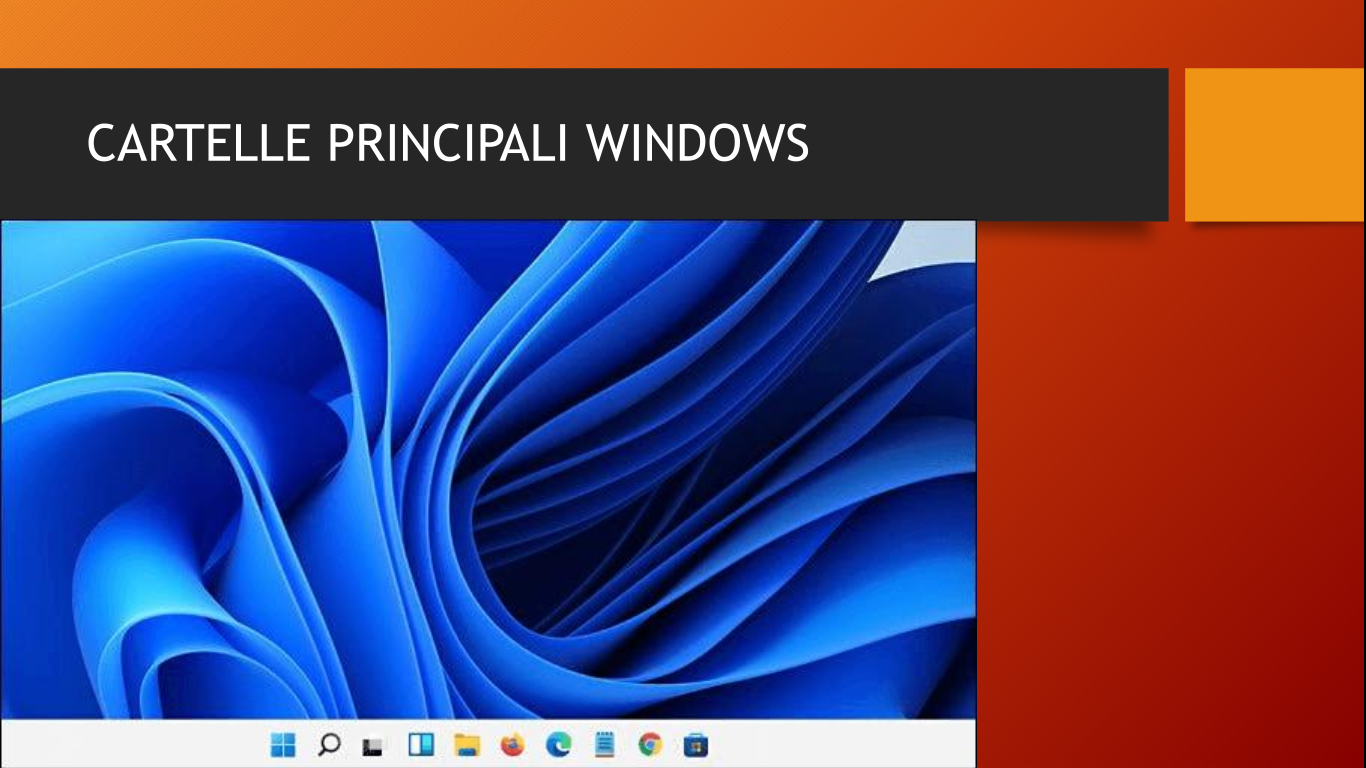
\includegraphics[width=\linewidth]{img/windows1.png}
        \caption{screenshot dell'interfaccia di \href{https://www.microsoft.com/}{Microsoft Windows}, modificato con \href{https://www.microsoft.com/it-it/microsoft-365/powerpoint}{PowerPoint}}
    \end{figure}}
    \only<2>{\begin{figure}
        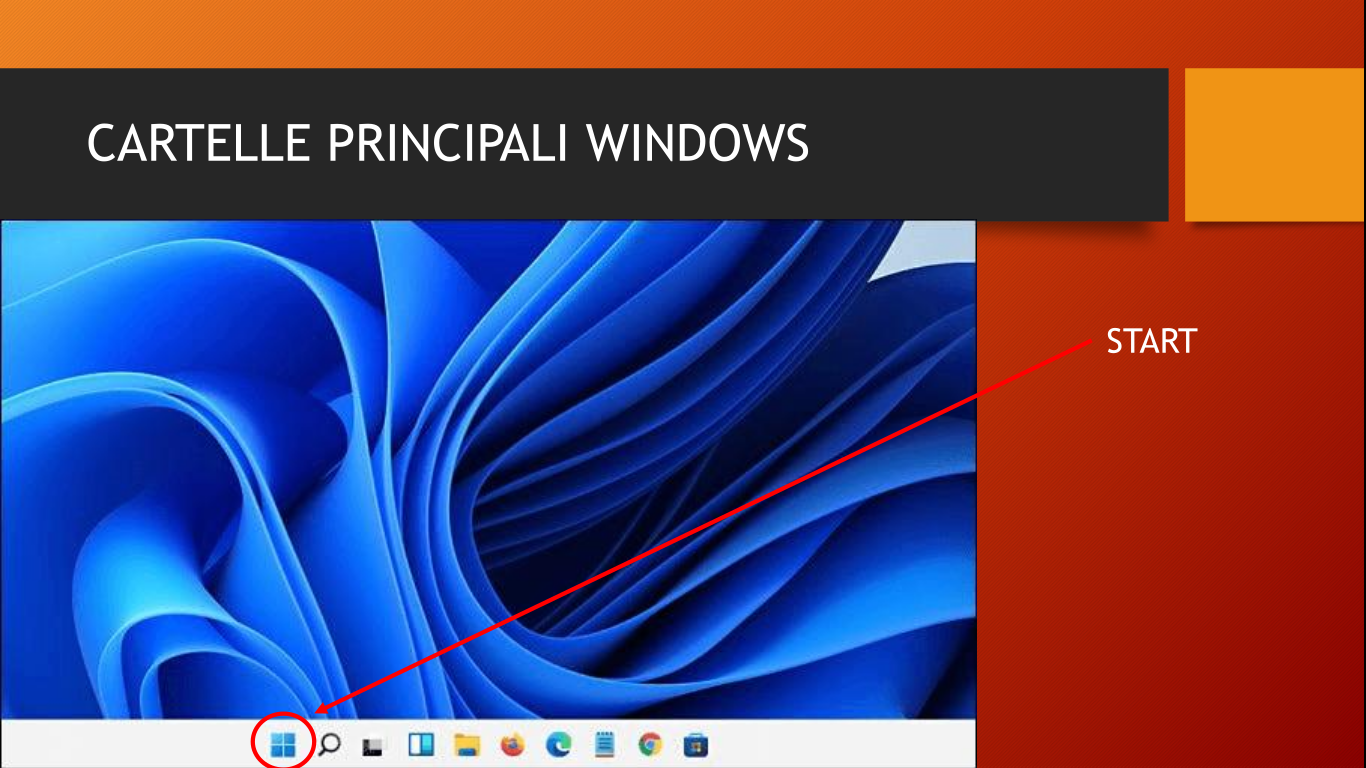
\includegraphics[width=\linewidth]{img/windows2.png}
        \caption{screenshot dell'interfaccia di \href{https://www.microsoft.com/}{Microsoft Windows}, modificato con \href{https://www.microsoft.com/it-it/microsoft-365/powerpoint}{PowerPoint}}
    \end{figure}}
    \only<3>{\begin{figure}
        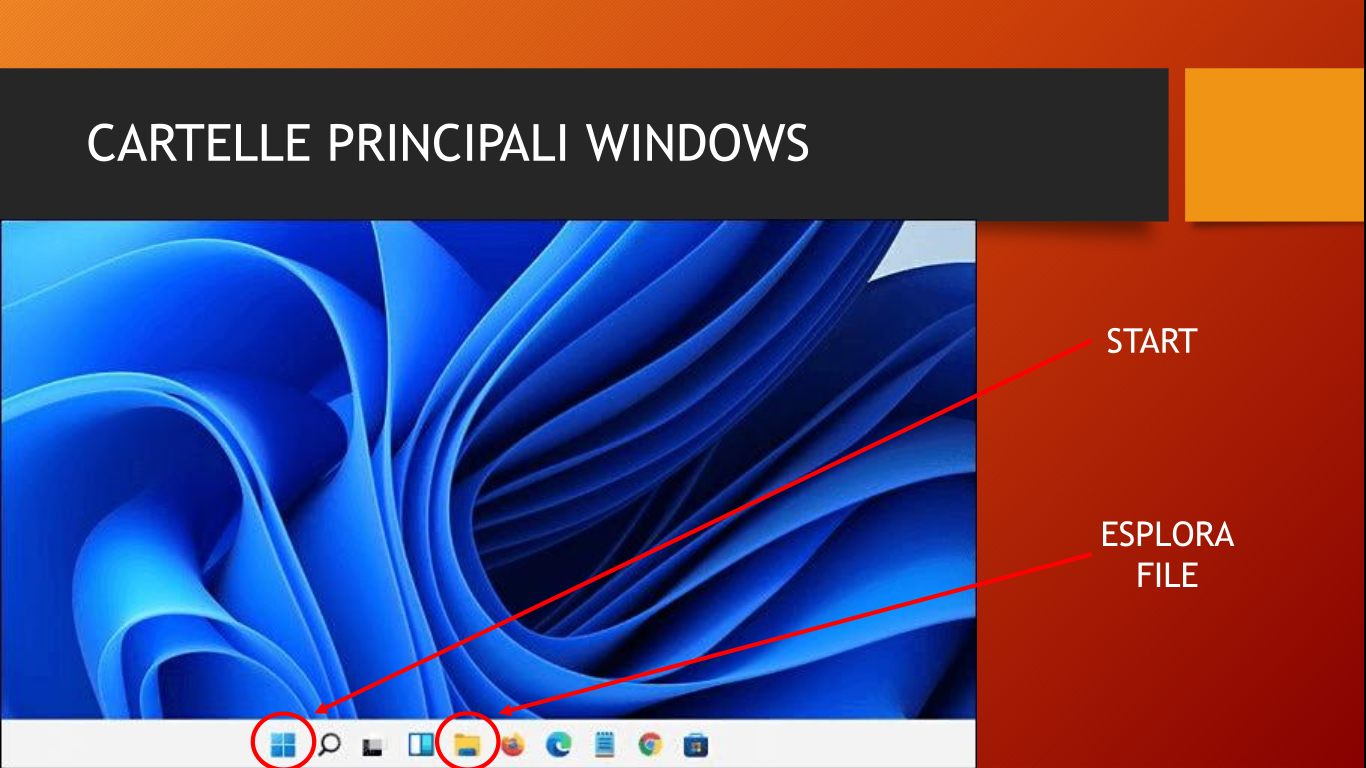
\includegraphics[width=\linewidth]{img/windows3.png}
        \caption{screenshot dell'interfaccia di \href{https://www.microsoft.com/}{Microsoft Windows}, modificato con \href{https://www.microsoft.com/it-it/microsoft-365/powerpoint}{PowerPoint}}
    \end{figure}}
\end{frame}

\begin{frame}{MICROSOFT WINDOWS}
    \only<1>{\begin{figure}
        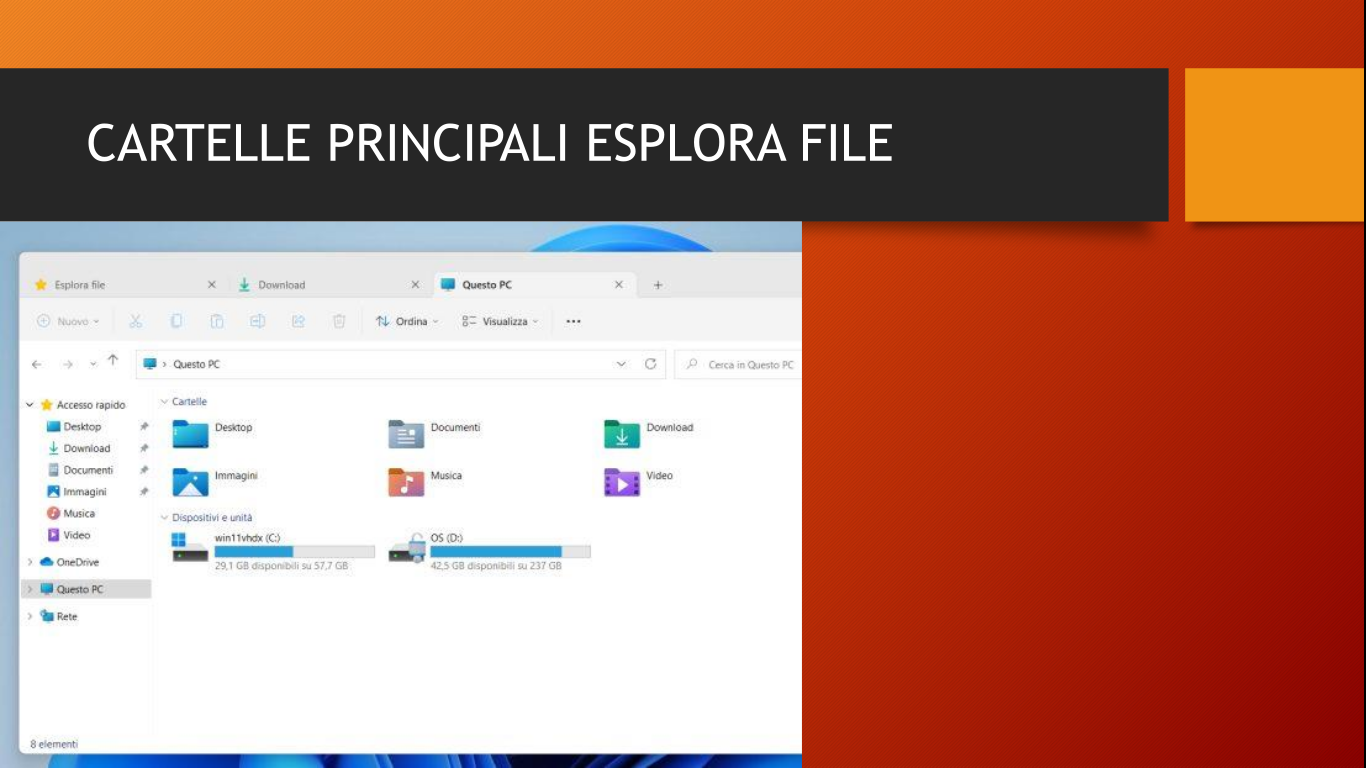
\includegraphics[width=\linewidth]{img/windows4.png}
        \caption{screenshot dell'interfaccia di \href{https://www.microsoft.com/}{Microsoft Windows}, modificato con \href{https://www.microsoft.com/it-it/microsoft-365/powerpoint}{PowerPoint}}
    \end{figure}}
    \only<2>{\begin{figure}
        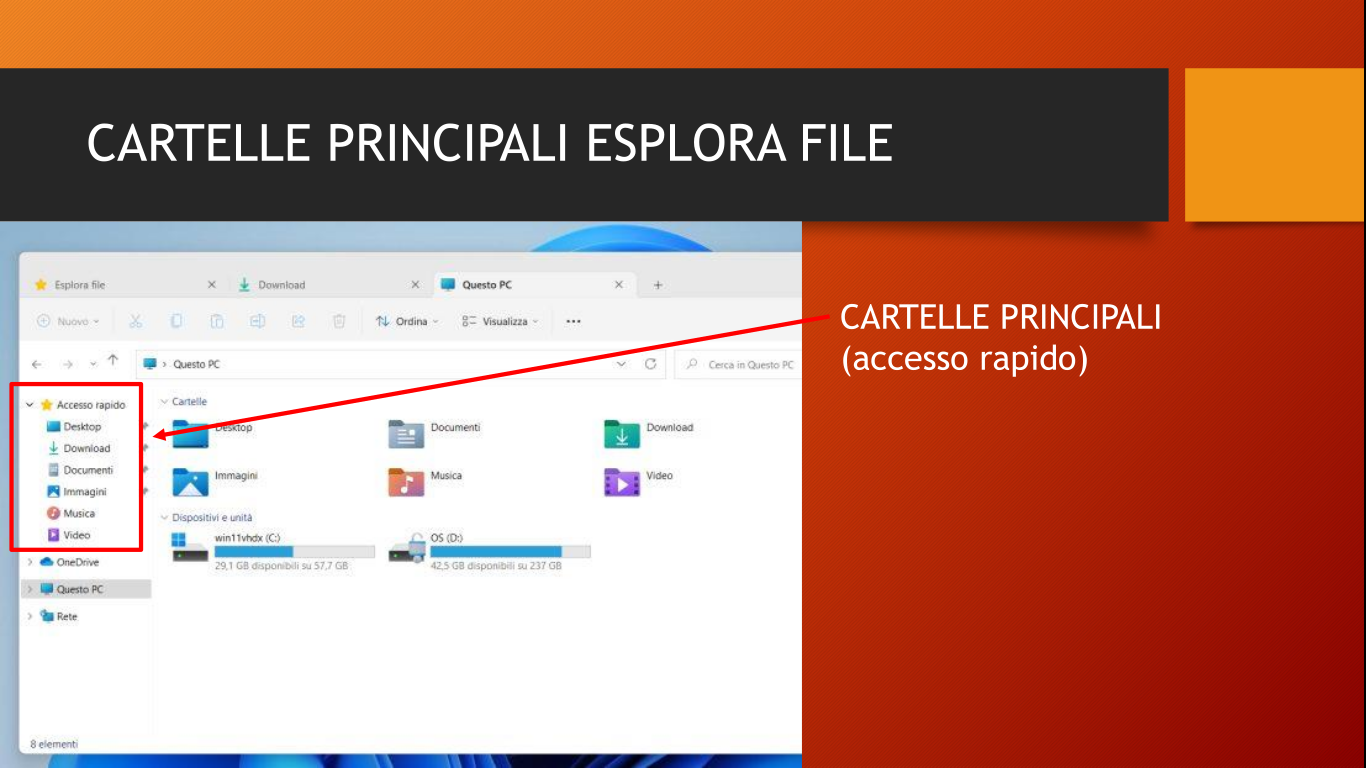
\includegraphics[width=\linewidth]{img/windows5.png}
        \caption{screenshot dell'interfaccia di \href{https://www.microsoft.com/}{Microsoft Windows}, modificato con \href{https://www.microsoft.com/it-it/microsoft-365/powerpoint}{PowerPoint}}
    \end{figure}}
    \only<3>{\begin{figure}
        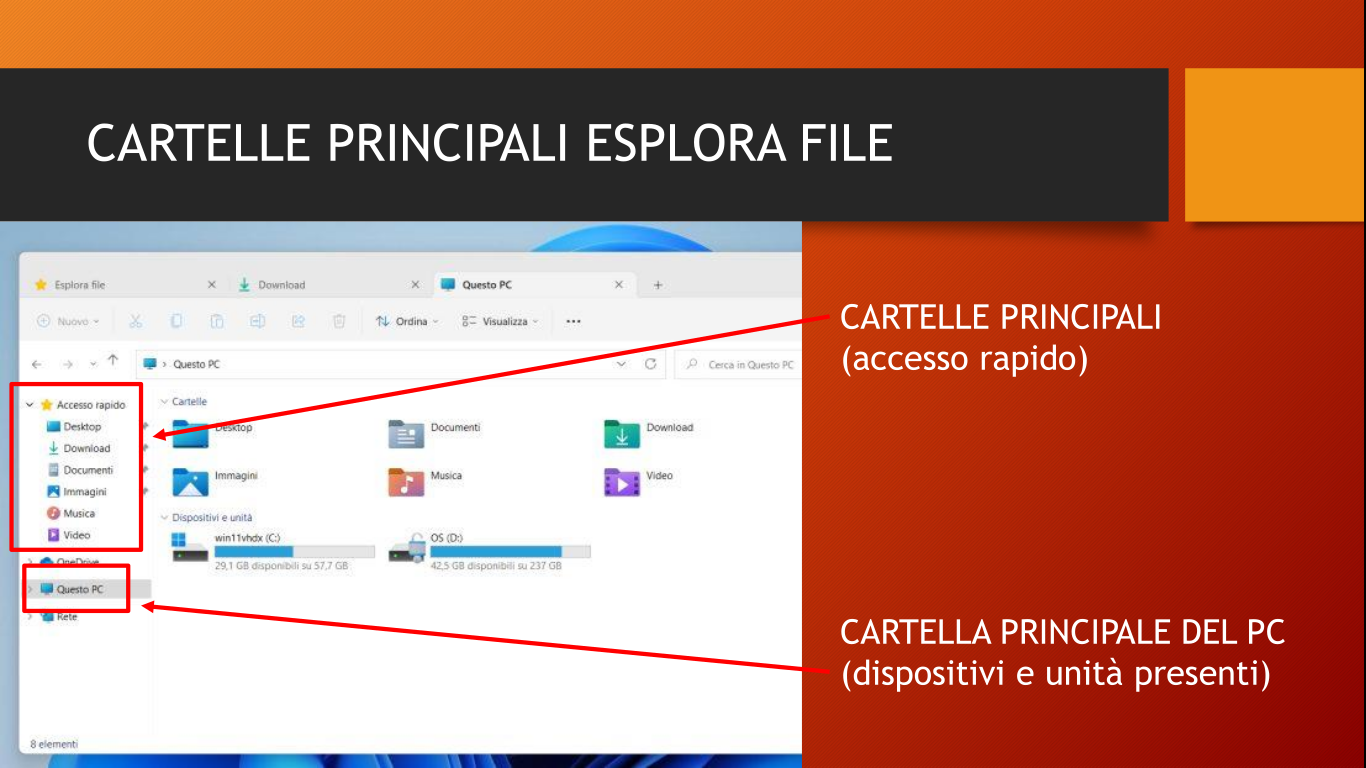
\includegraphics[width=\linewidth]{img/windows6.png}
        \caption{screenshot dell'interfaccia di \href{https://www.microsoft.com/}{Microsoft Windows}, modificato con \href{https://www.microsoft.com/it-it/microsoft-365/powerpoint}{PowerPoint}}
    \end{figure}}
    \only<4>{\begin{figure}
        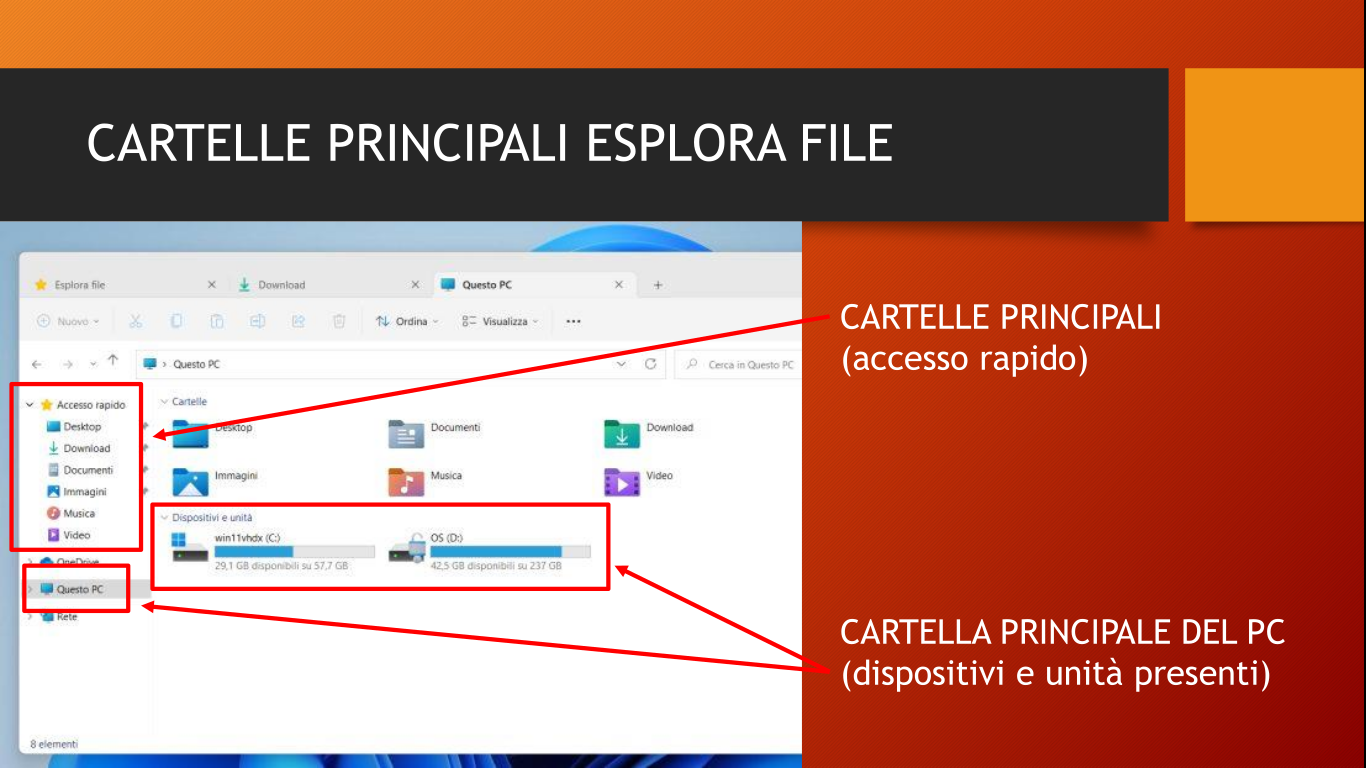
\includegraphics[width=\linewidth]{img/windows7.png}
        \caption{screenshot dell'interfaccia di \href{https://www.microsoft.com/}{Microsoft Windows}, modificato con \href{https://www.microsoft.com/it-it/microsoft-365/powerpoint}{PowerPoint}}
    \end{figure}}
\end{frame}

\begin{frame}{MICROSOFT WINDOWS}
    \only<1>{\begin{figure}
        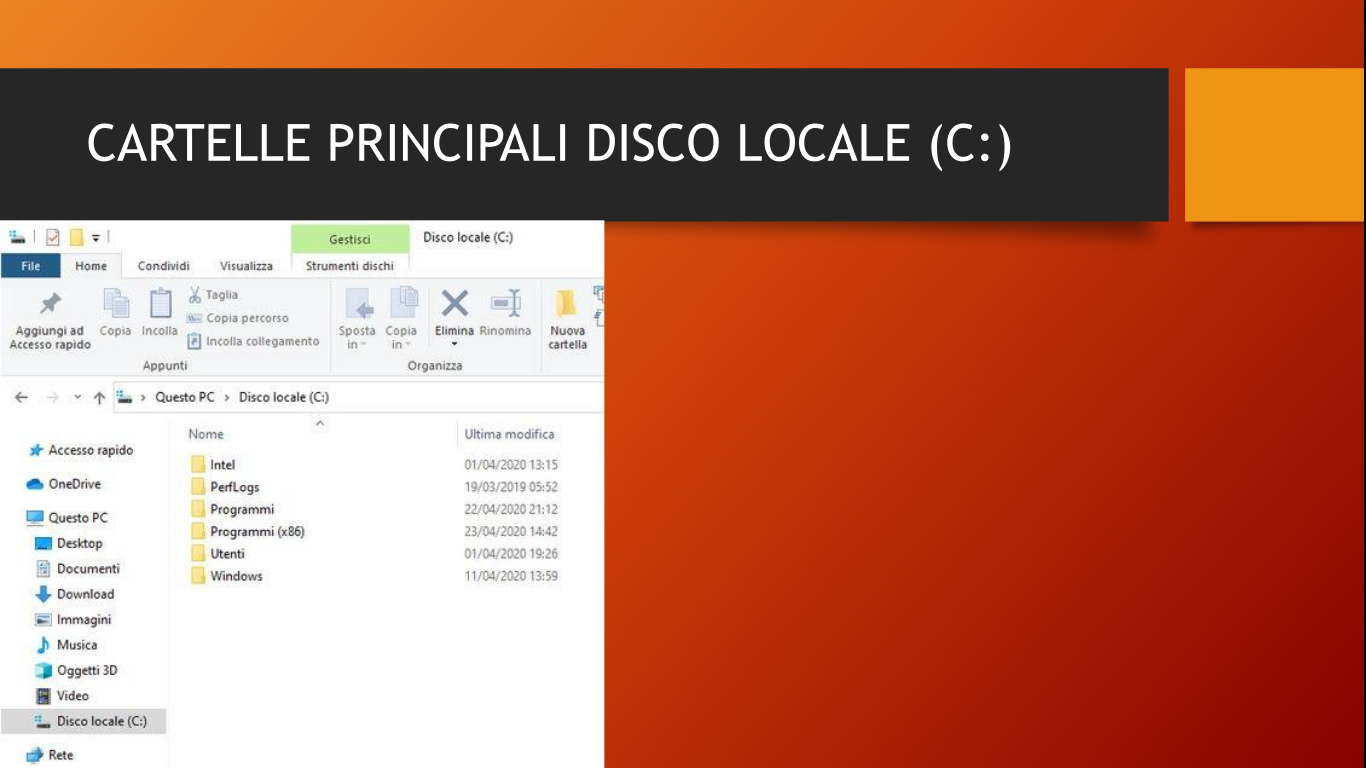
\includegraphics[width=\linewidth]{img/windows8.png}
        \caption{screenshot dell'interfaccia di \href{https://www.microsoft.com/}{Microsoft Windows}, modificato con \href{https://www.microsoft.com/it-it/microsoft-365/powerpoint}{PowerPoint}}
    \end{figure}}
    \only<2>{\begin{figure}
        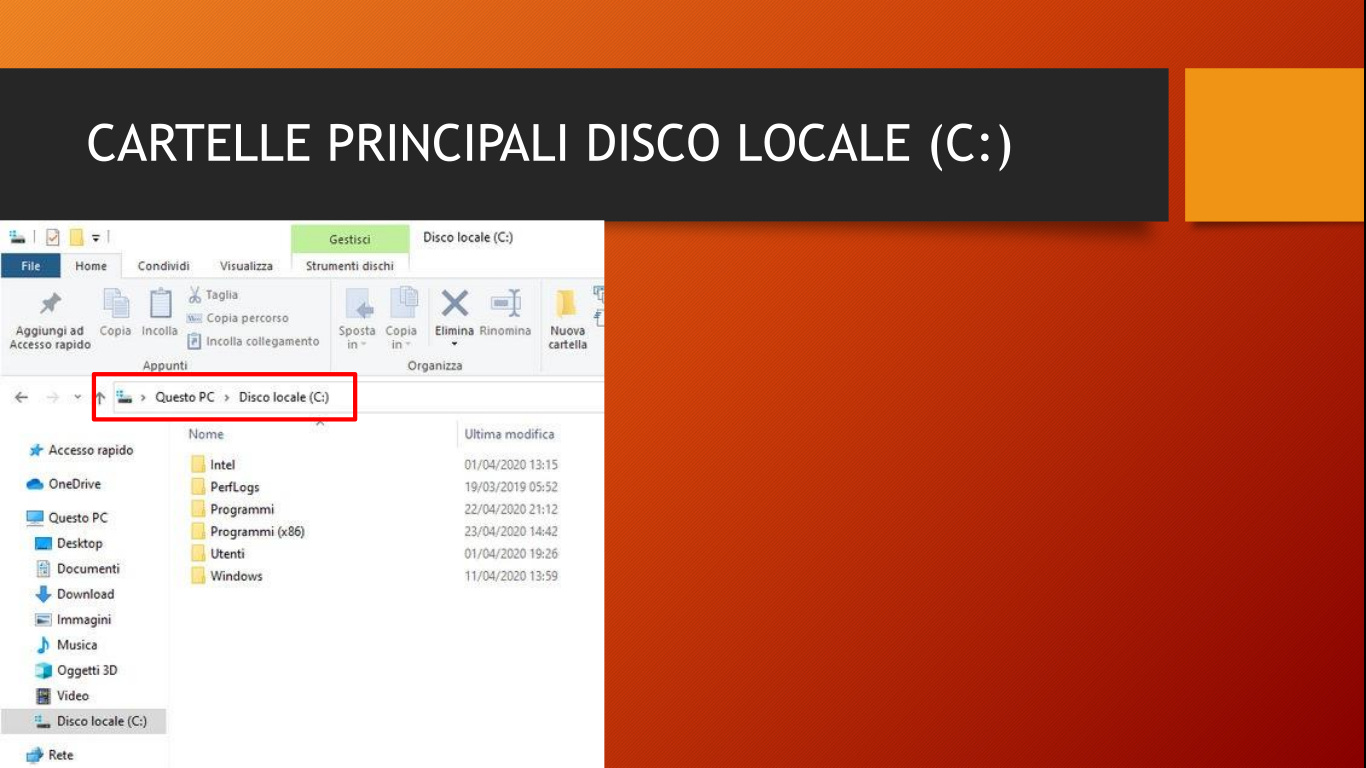
\includegraphics[width=\linewidth]{img/windows9.png}
        \caption{screenshot dell'interfaccia di \href{https://www.microsoft.com/}{Microsoft Windows}, modificato con \href{https://www.microsoft.com/it-it/microsoft-365/powerpoint}{PowerPoint}}
    \end{figure}}
    \only<3>{\begin{figure}
        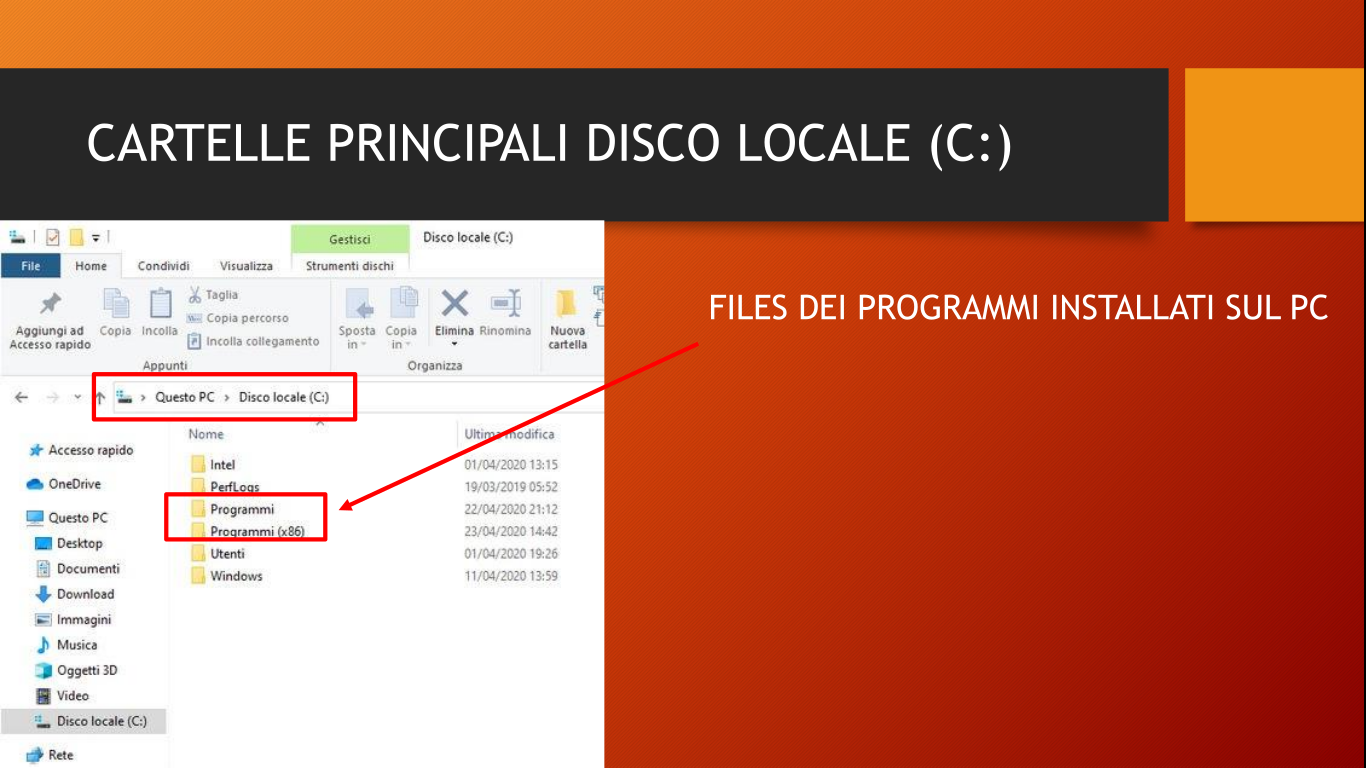
\includegraphics[width=\linewidth]{img/windows10.png}
        \caption{screenshot dell'interfaccia di \href{https://www.microsoft.com/}{Microsoft Windows}, modificato con \href{https://www.microsoft.com/it-it/microsoft-365/powerpoint}{PowerPoint}}
    \end{figure}}
    \only<4>{\begin{figure}
        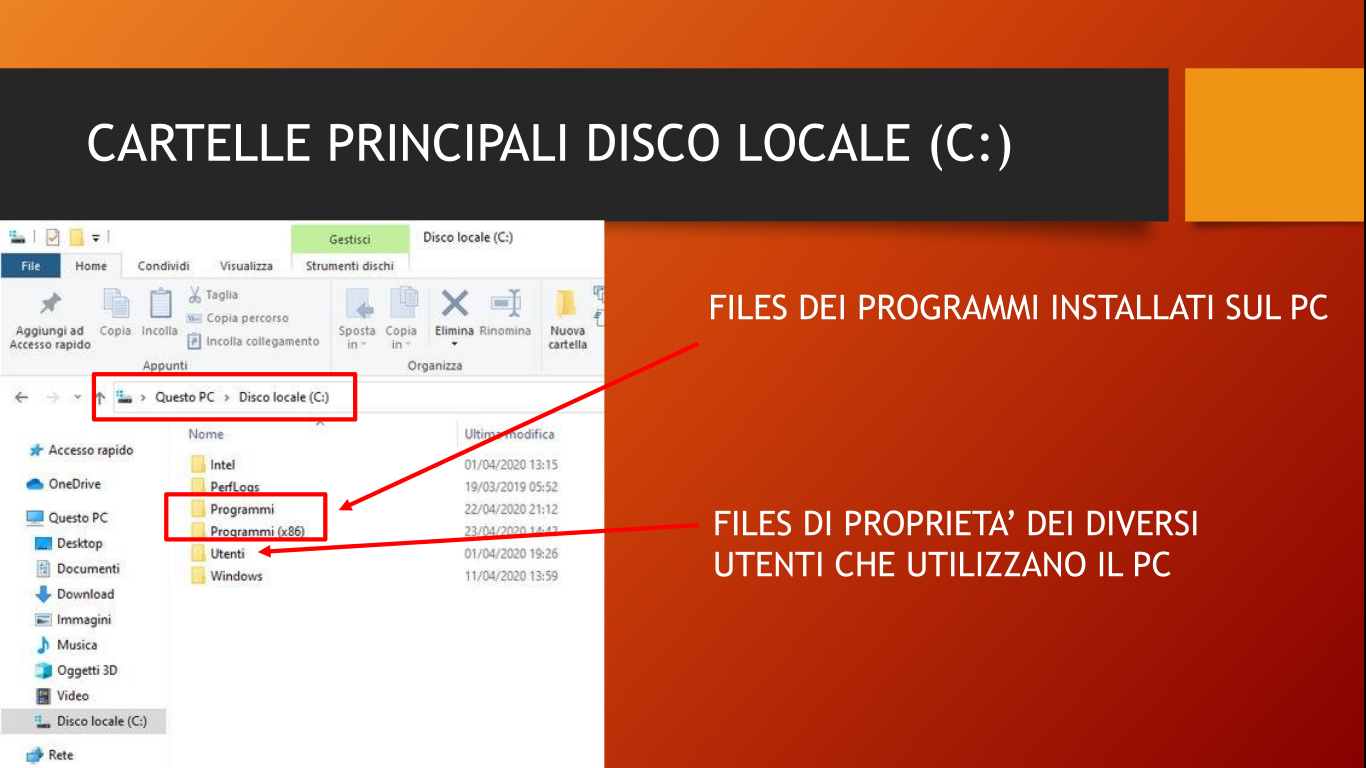
\includegraphics[width=\linewidth]{img/windows11.png}
        \caption{screenshot dell'interfaccia di \href{https://www.microsoft.com/}{Microsoft Windows}, modificato con \href{https://www.microsoft.com/it-it/microsoft-365/powerpoint}{PowerPoint}}
    \end{figure}}
    \only<5>{\begin{figure}
        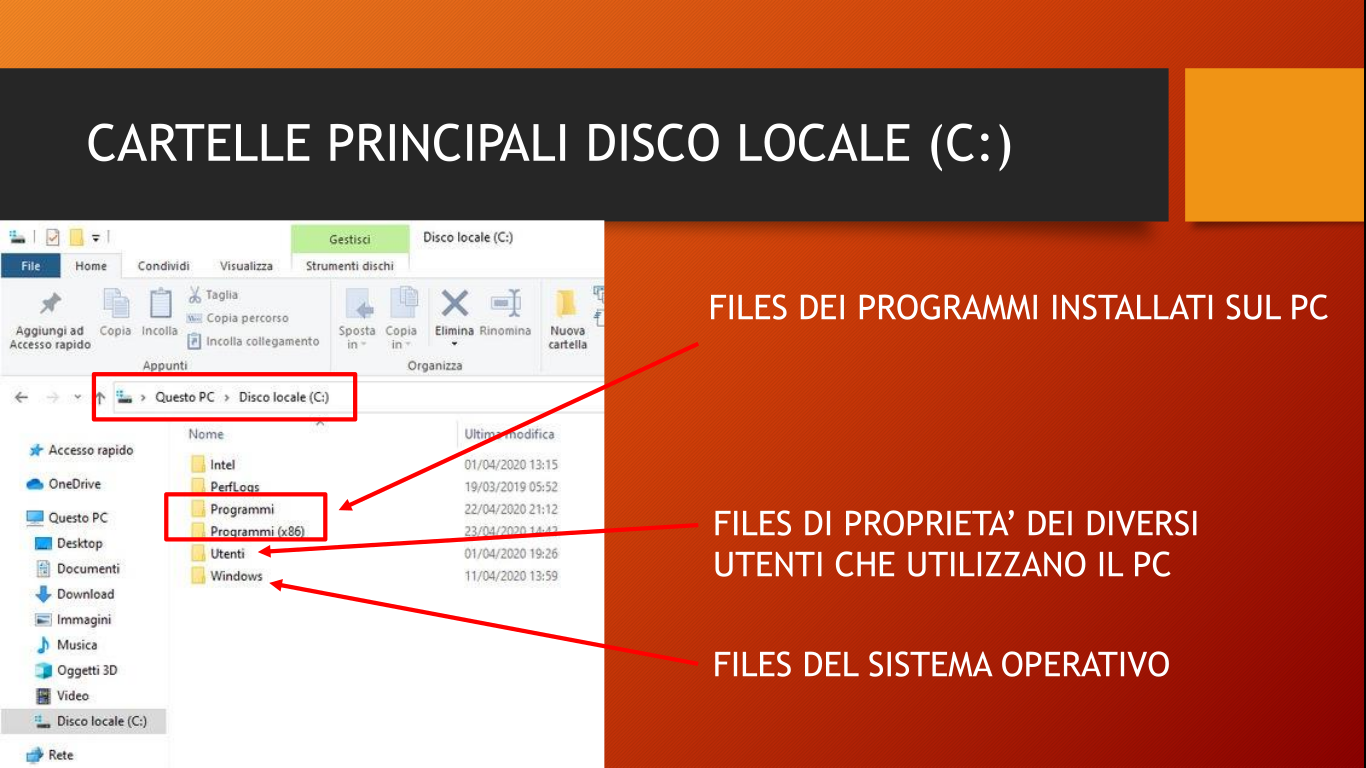
\includegraphics[width=\linewidth]{img/windows12.png}
        \caption{screenshot dell'interfaccia di \href{https://www.microsoft.com/}{Microsoft Windows}, modificato con \href{https://www.microsoft.com/it-it/microsoft-365/powerpoint}{PowerPoint}}
    \end{figure}}
\end{frame}

\begin{frame}{MICROSOFT WINDOWS}
    \begin{figure}
        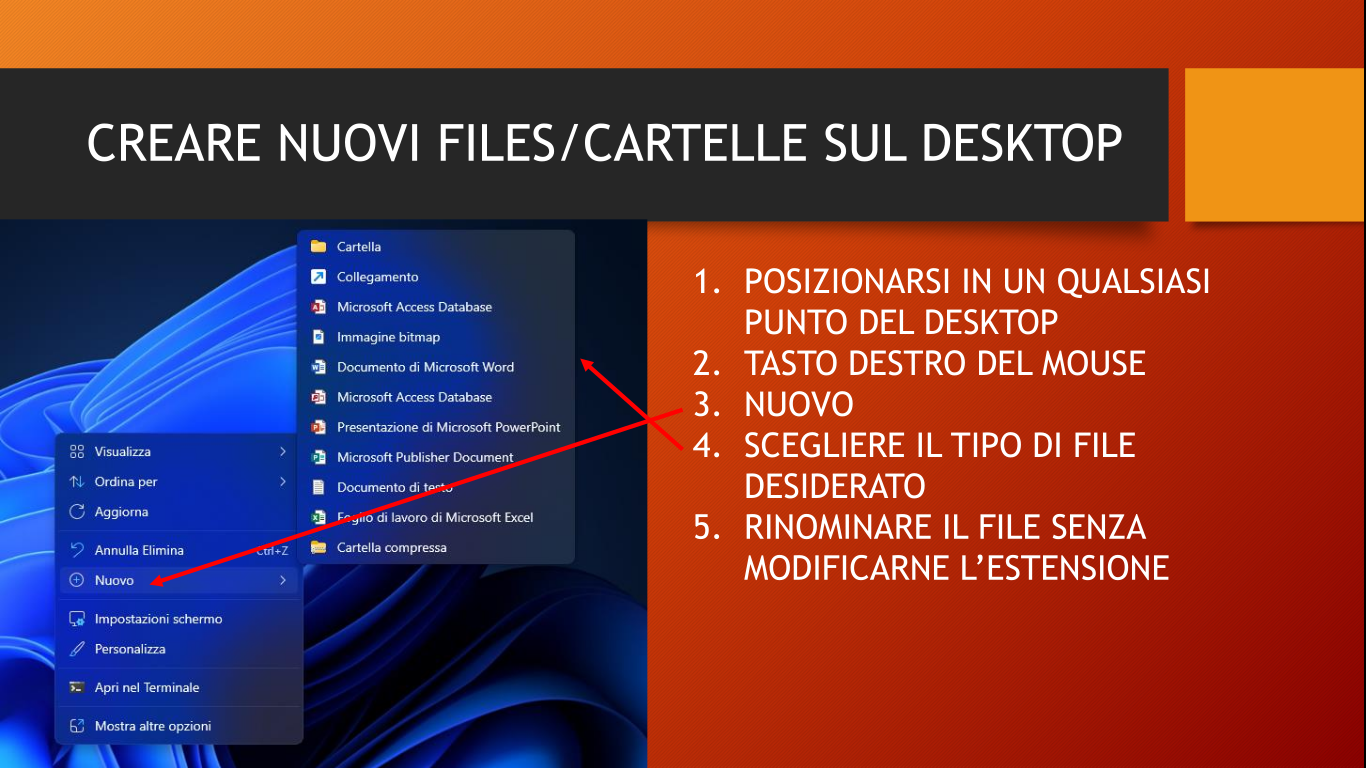
\includegraphics[width=\linewidth]{img/windows13.png}
        \caption{screenshot dell'interfaccia di \href{https://www.microsoft.com/}{Microsoft Windows}, modificato con \href{https://www.microsoft.com/it-it/microsoft-365/powerpoint}{PowerPoint}}
    \end{figure}
\end{frame}

\begin{frame}{MICROSOFT WINDOWS}
    \begin{figure}
        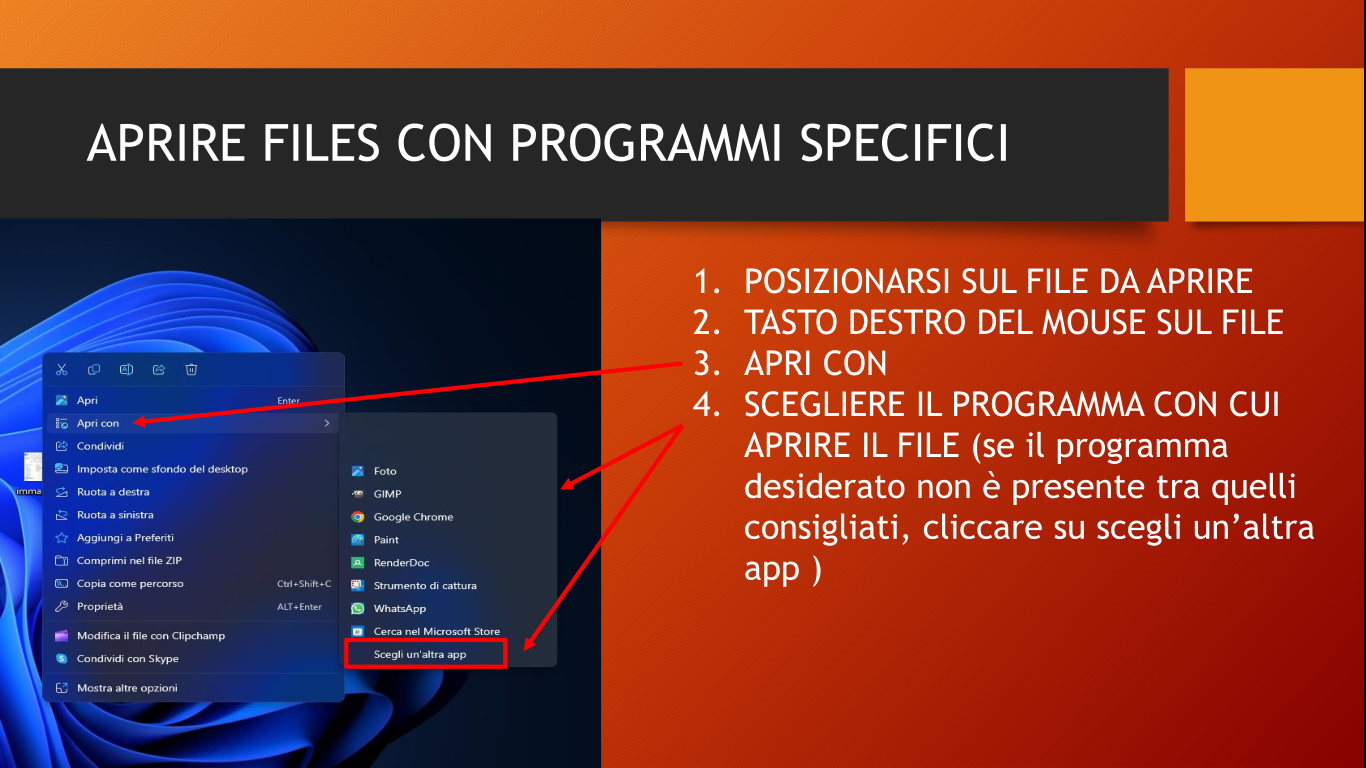
\includegraphics[width=\linewidth]{img/windows14.png}
        \caption{screenshot dell'interfaccia di \href{https://www.microsoft.com/}{Microsoft Windows}, modificato con \href{https://www.microsoft.com/it-it/microsoft-365/powerpoint}{PowerPoint}}
    \end{figure}
\end{frame}

\section{DRIVE}

\begin{frame}{GOOGLE DRIVE}
    \only<1>{\begin{figure}
        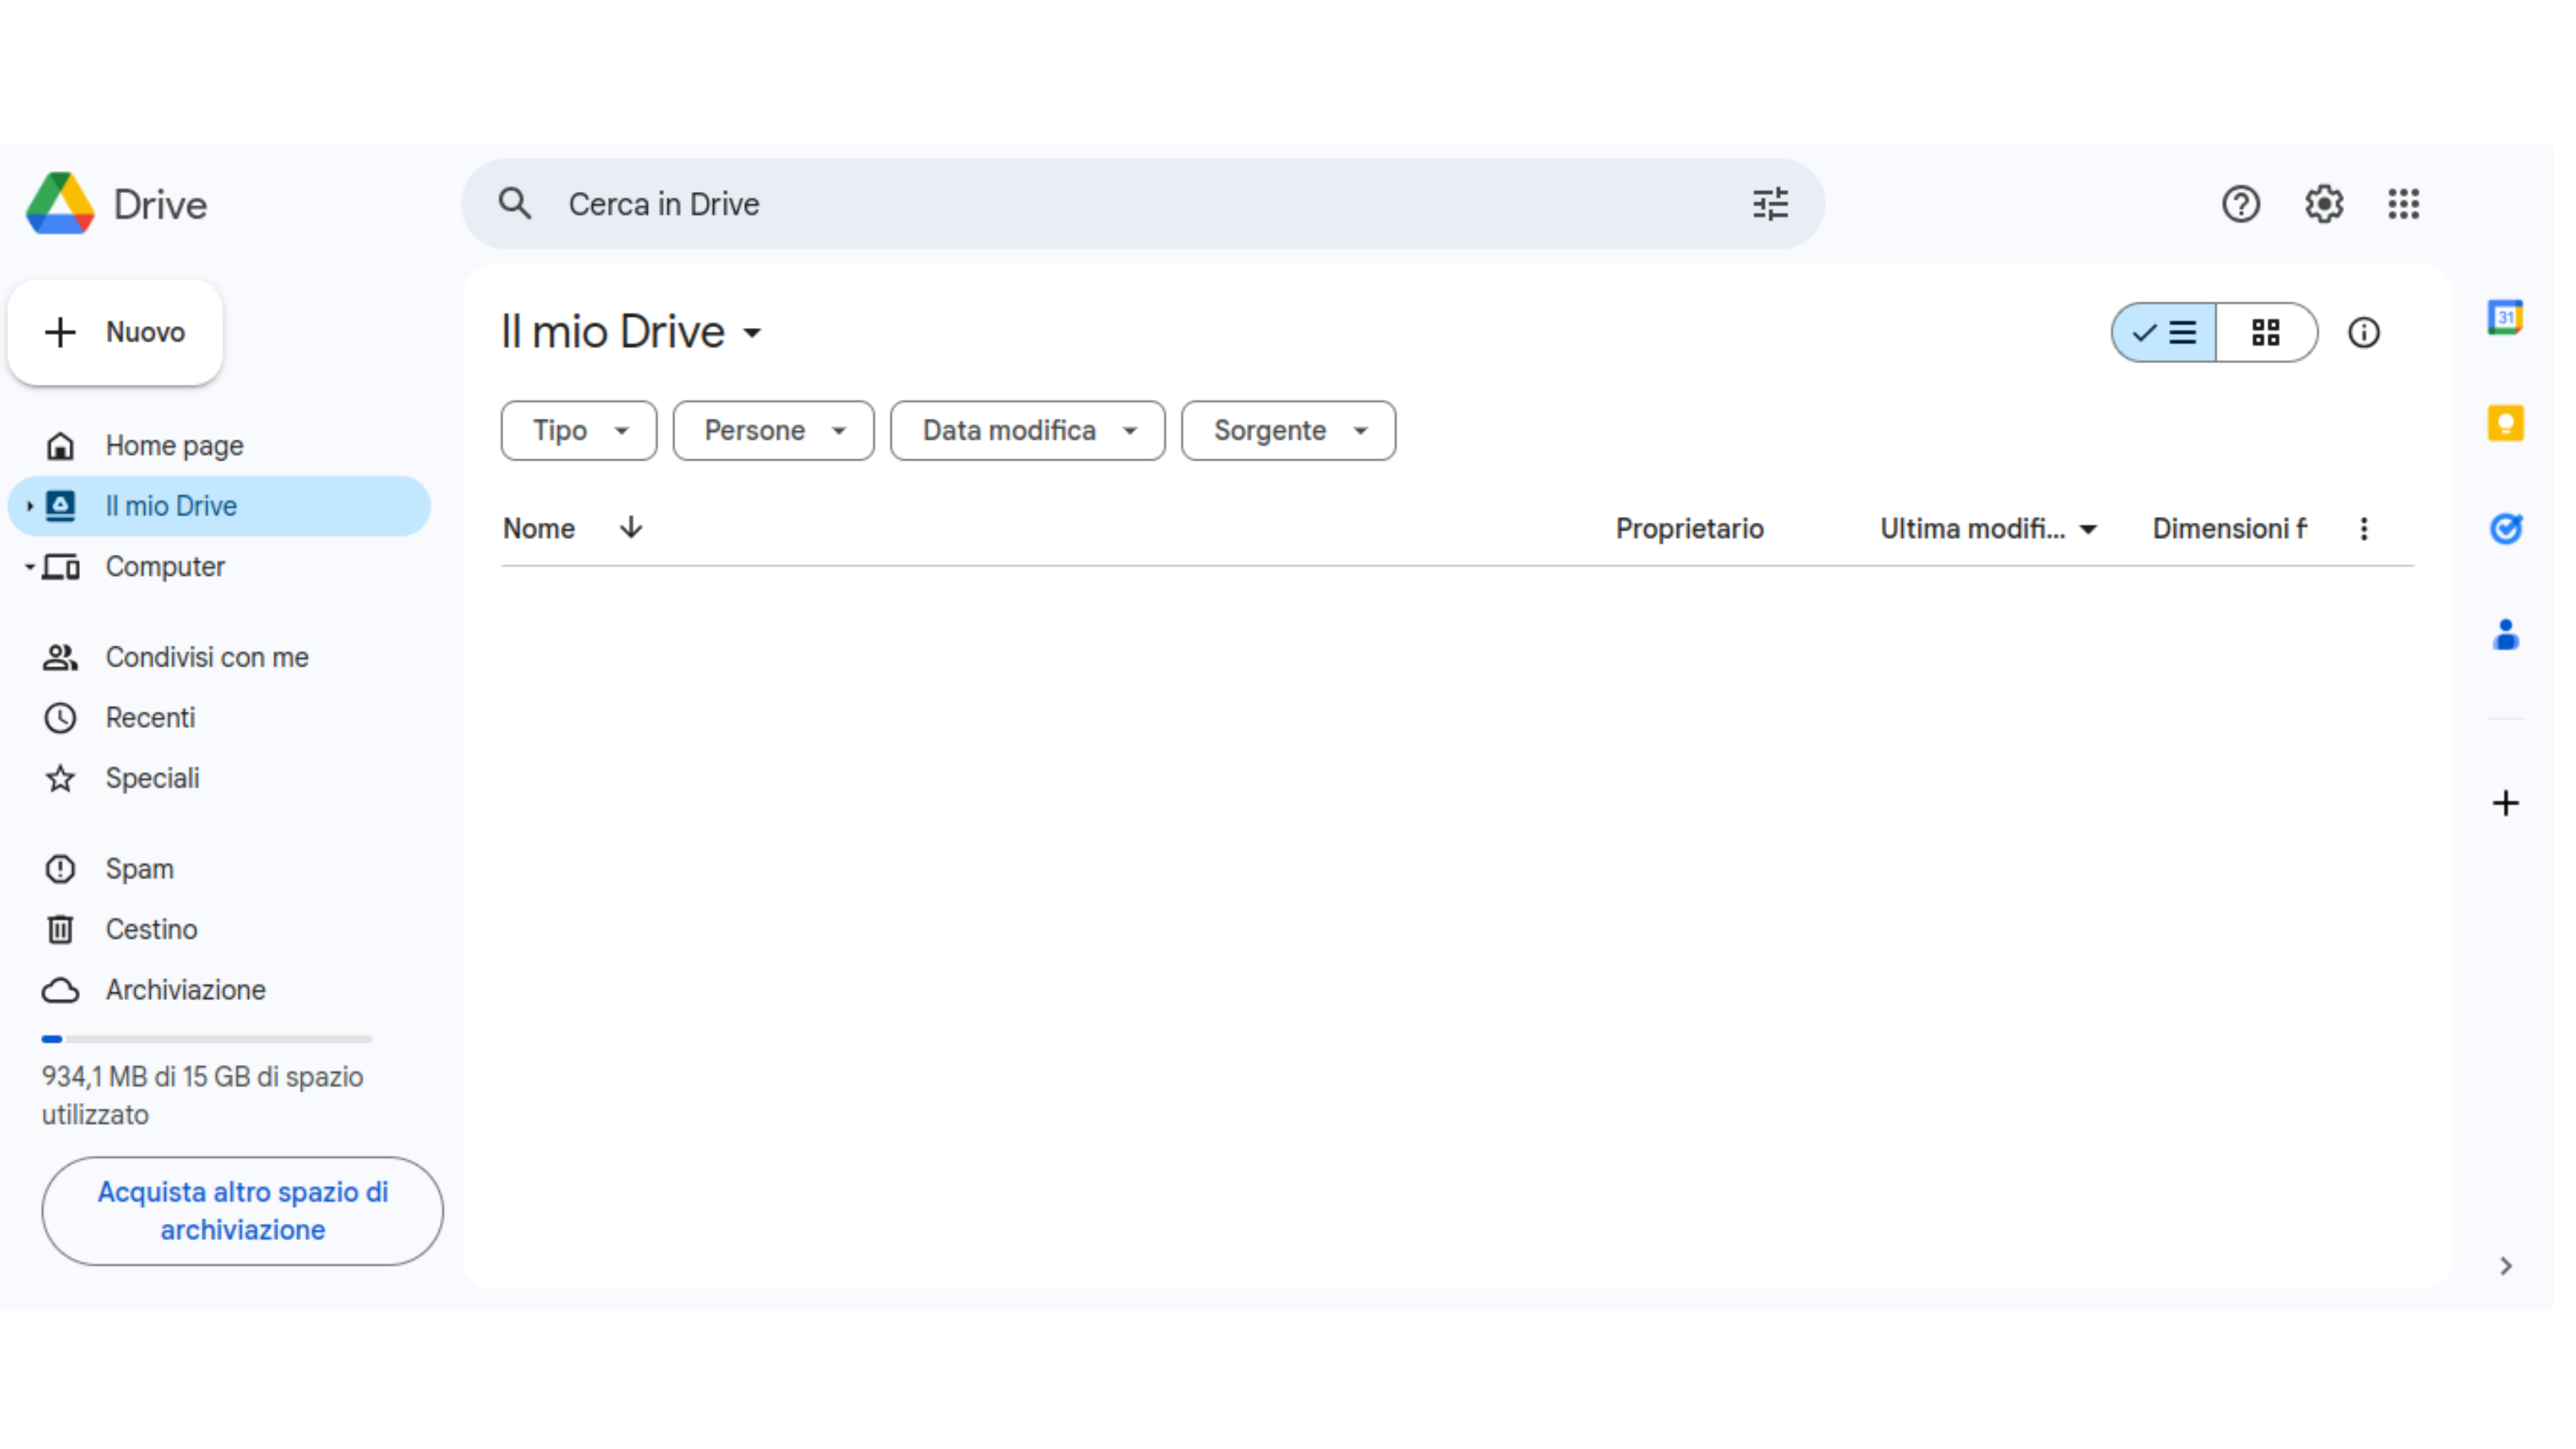
\includegraphics[width=\linewidth]{img/drive1.png}
        \caption{{screenshot della homepage di \href{https://drive.google.com}{Google Drive}}, modificato con \href{https://www.canva.com}{Canva}}
    \end{figure}}
    \only<2>{\begin{figure}
        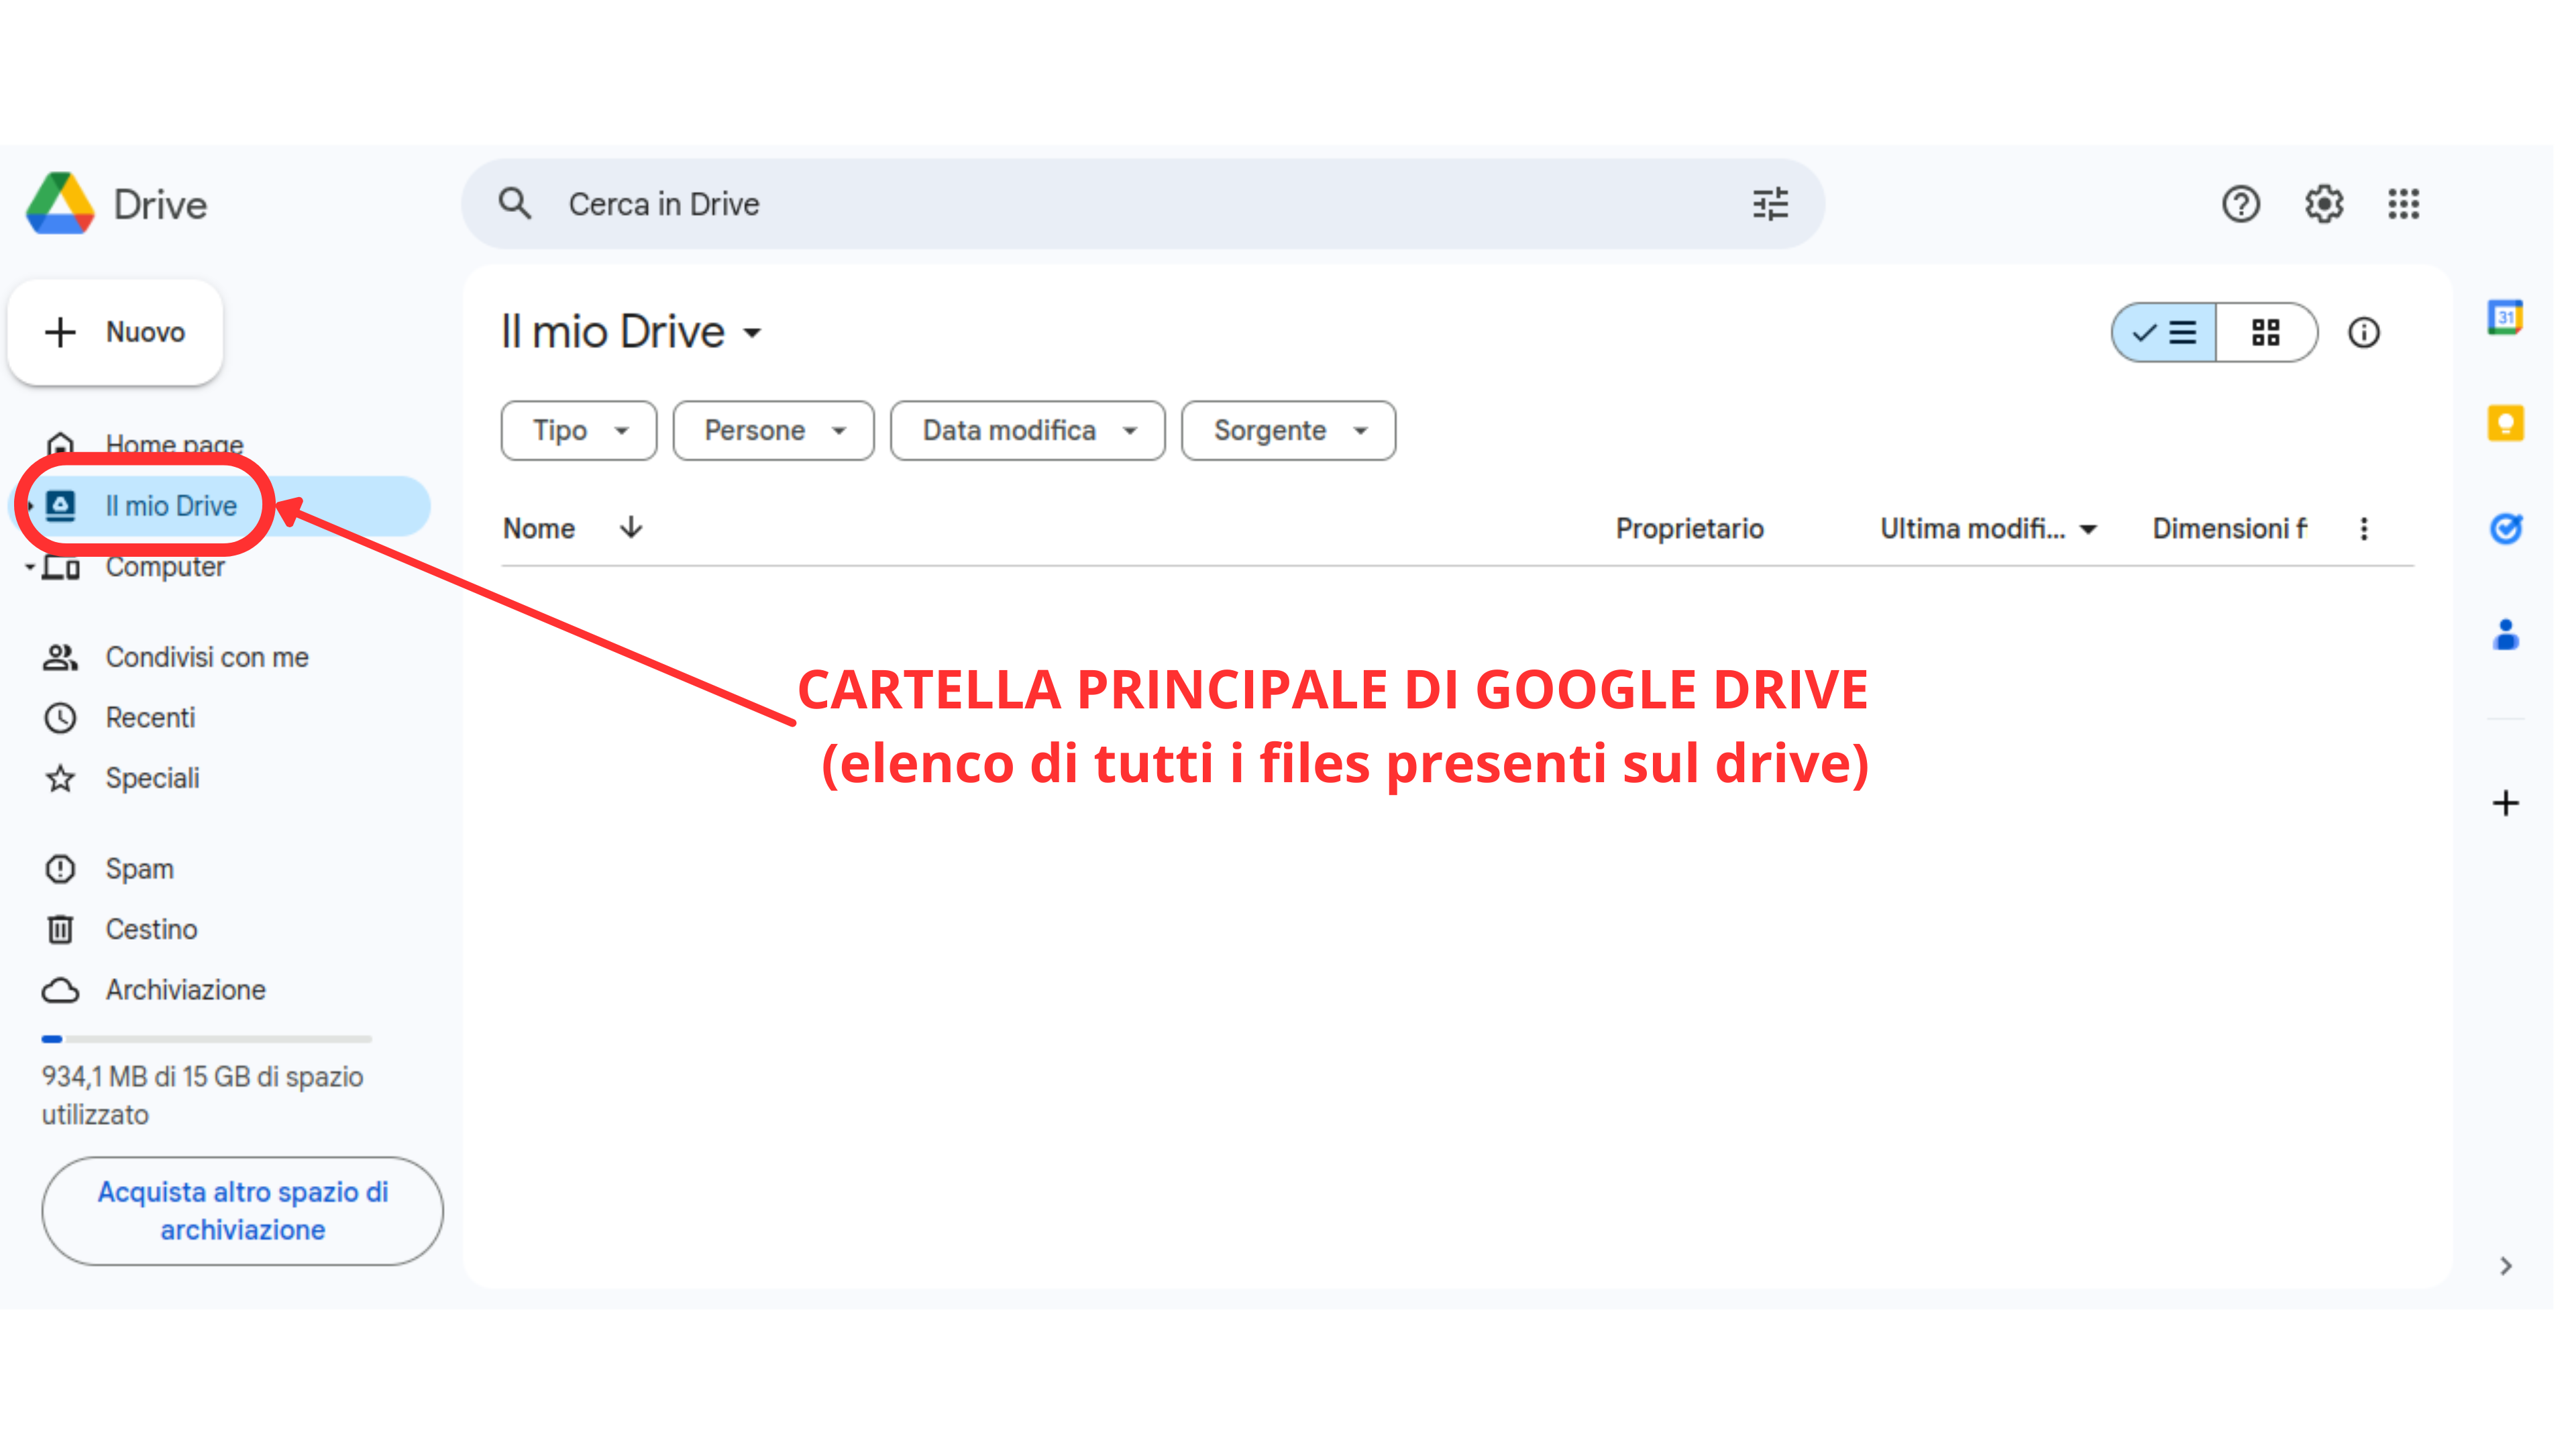
\includegraphics[width=\linewidth]{img/drive2.png}
        \caption{{screenshot della homepage di \href{https://drive.google.com}{Google Drive}}, modificato con \href{https://www.canva.com}{Canva}}
    \end{figure}}
    \only<3>{\begin{figure}
        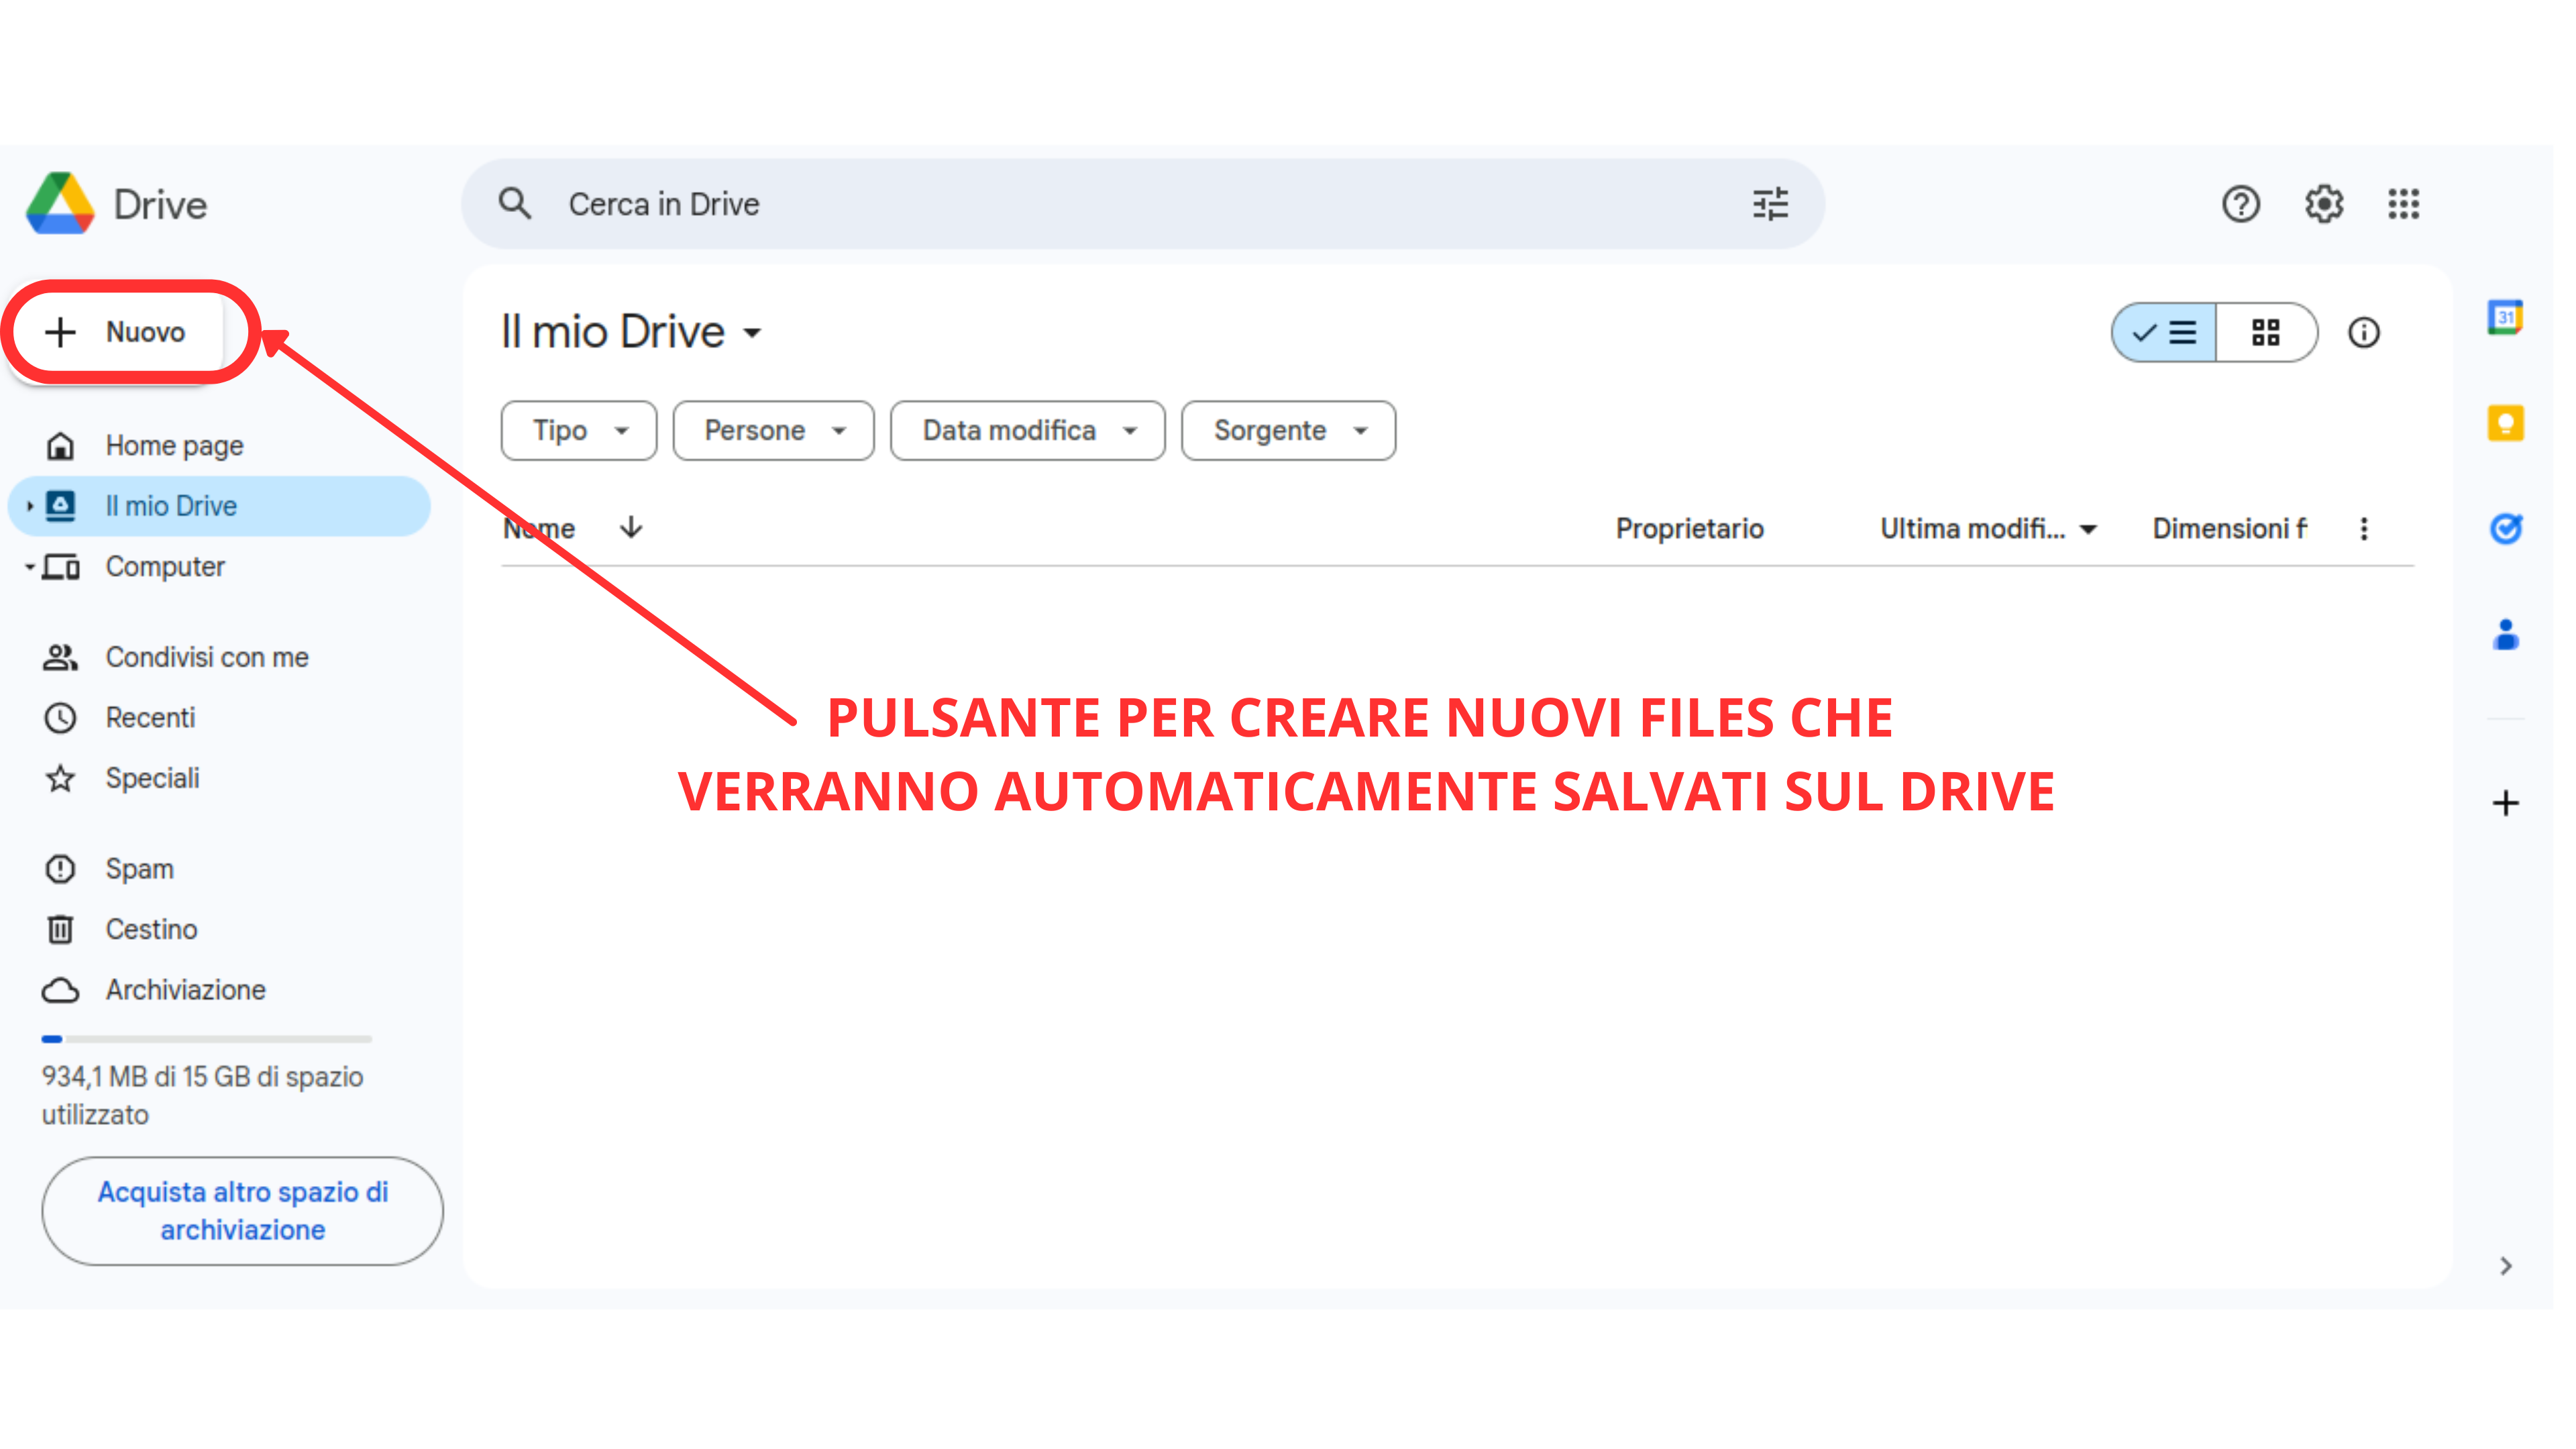
\includegraphics[width=\linewidth]{img/drive3.png}
        \caption{{screenshot della homepage di \href{https://drive.google.com}{Google Drive}}, modificato con \href{https://www.canva.com}{Canva}}
    \end{figure}}
    \only<4>{\begin{figure}
        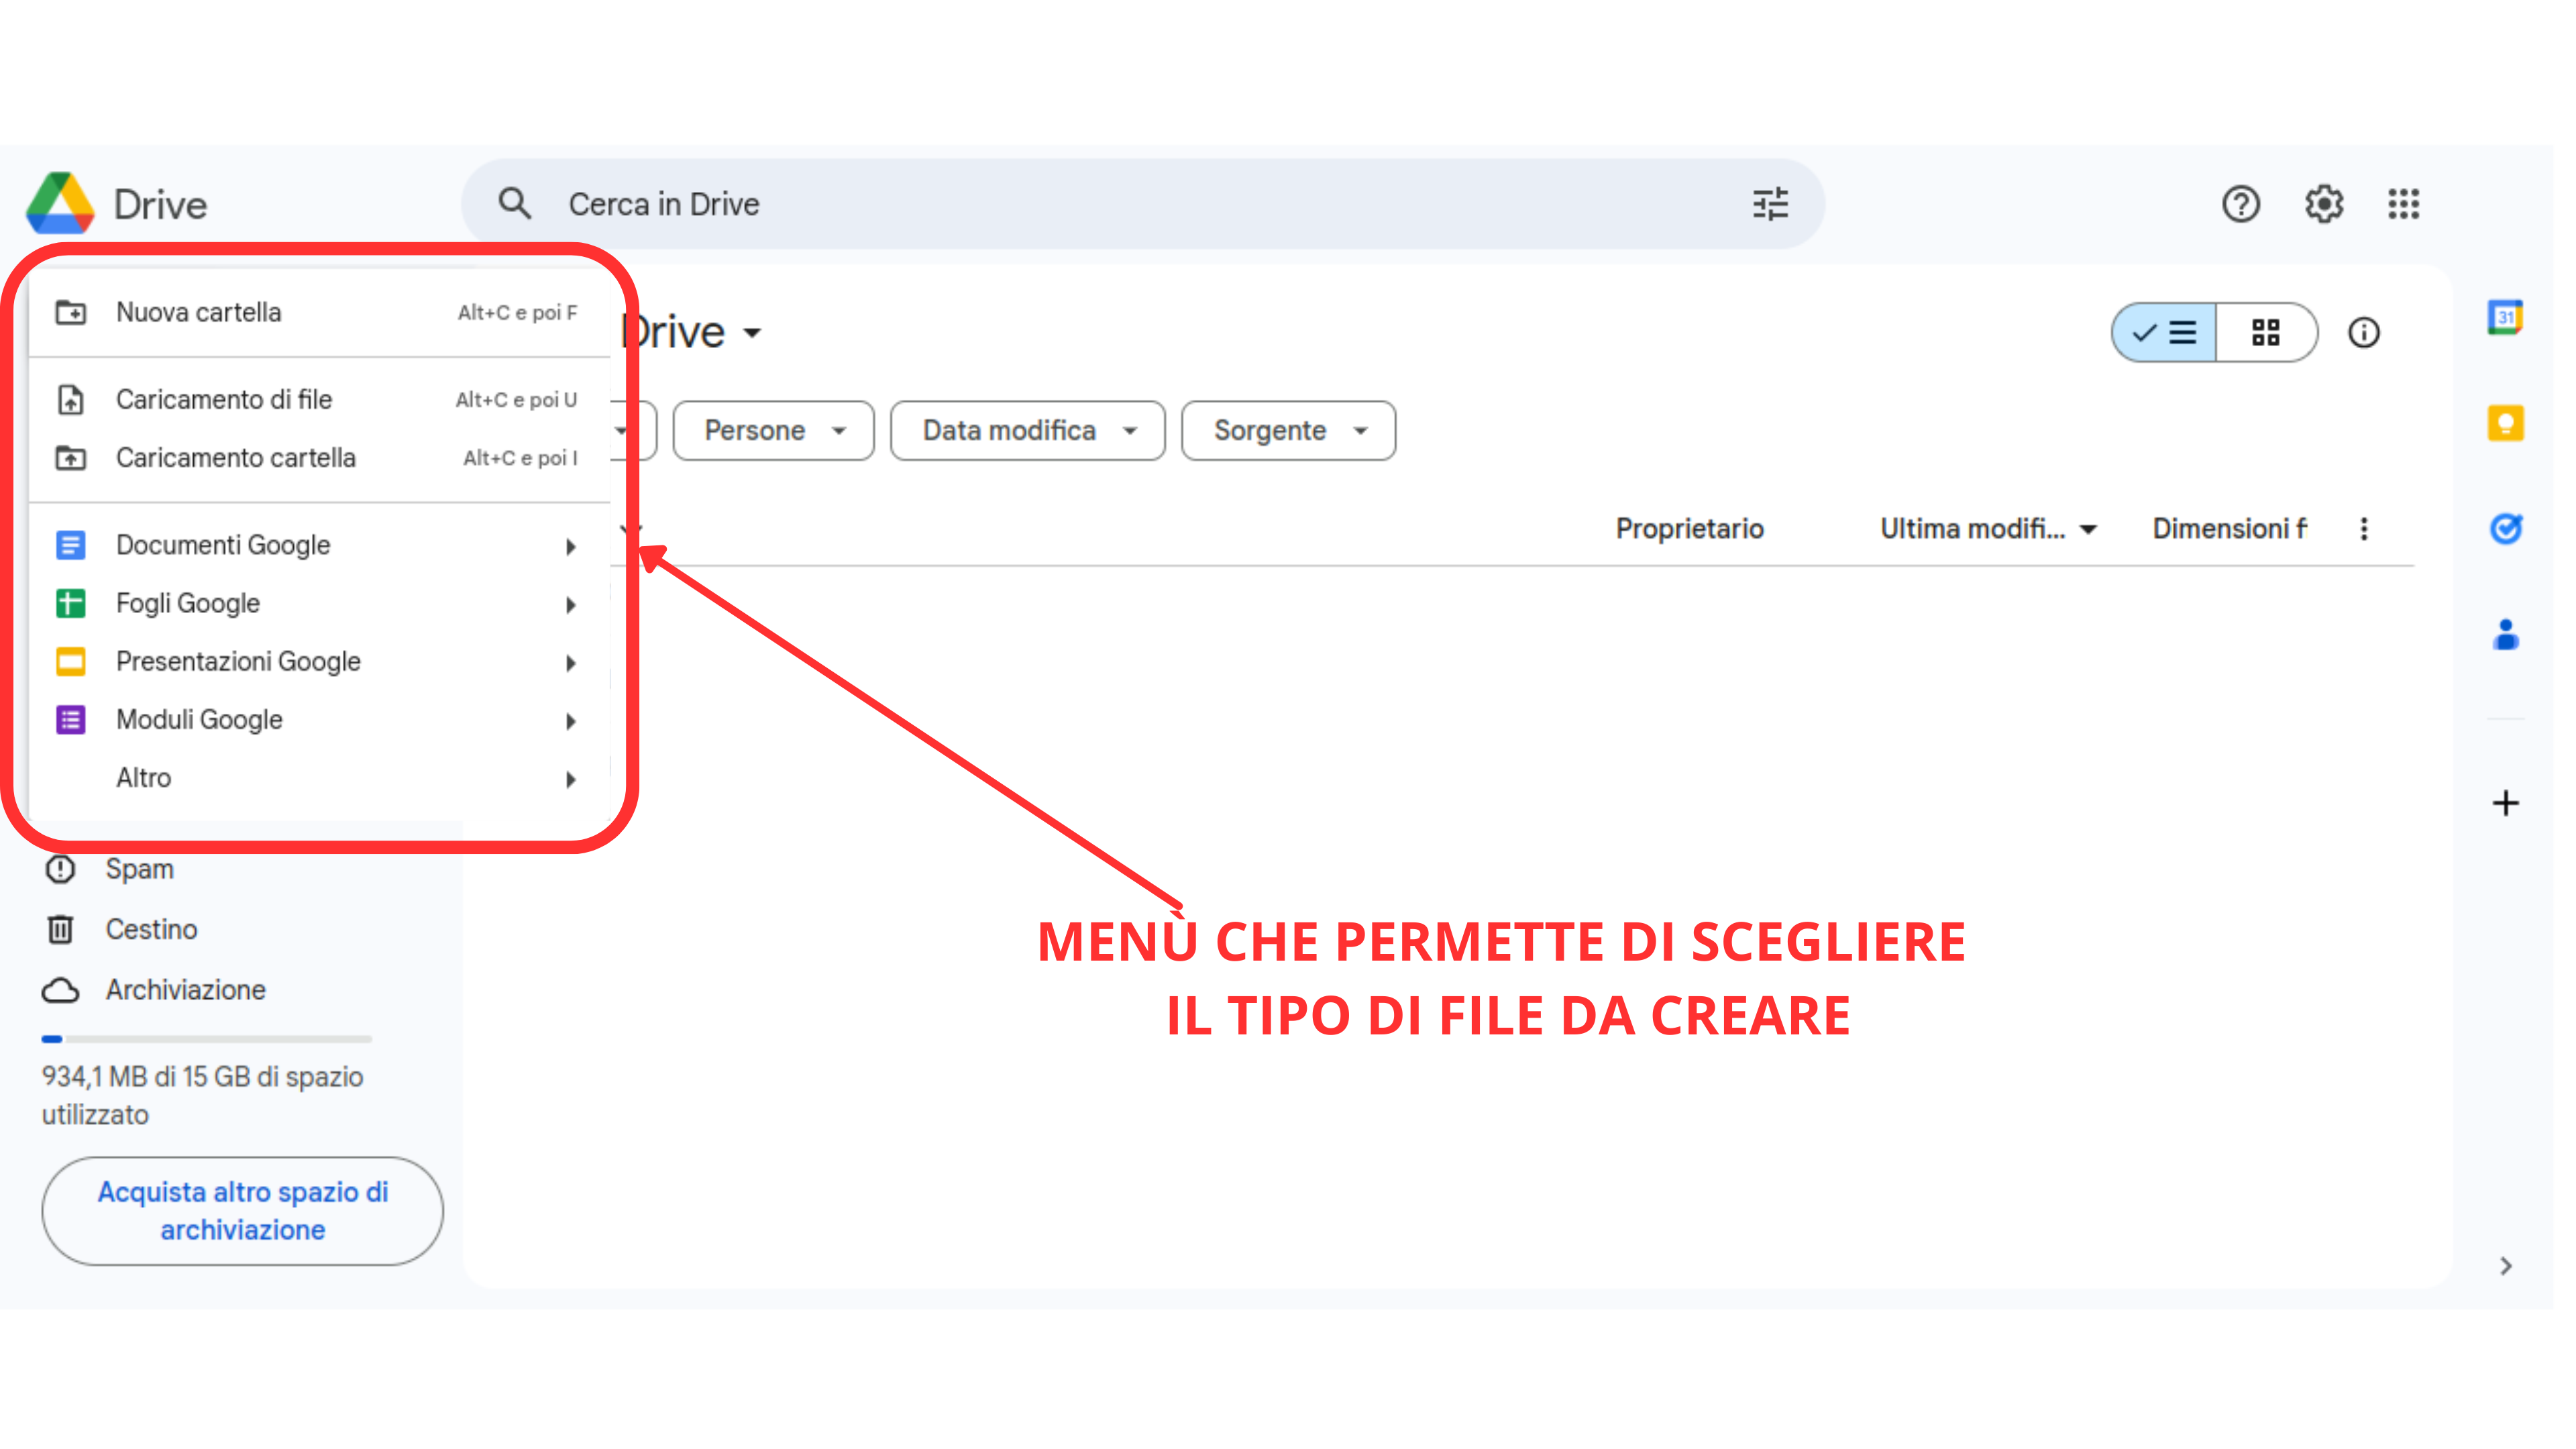
\includegraphics[width=\linewidth]{img/drive4.png}
        \caption{{screenshot della homepage di \href{https://drive.google.com}{Google Drive}}, modificato con \href{https://www.canva.com}{Canva}}
    \end{figure}}
\end{frame}

\section{MAIL}

\begin{frame}{GOOGLE MAIL}
    \only<1>{\begin{figure}
        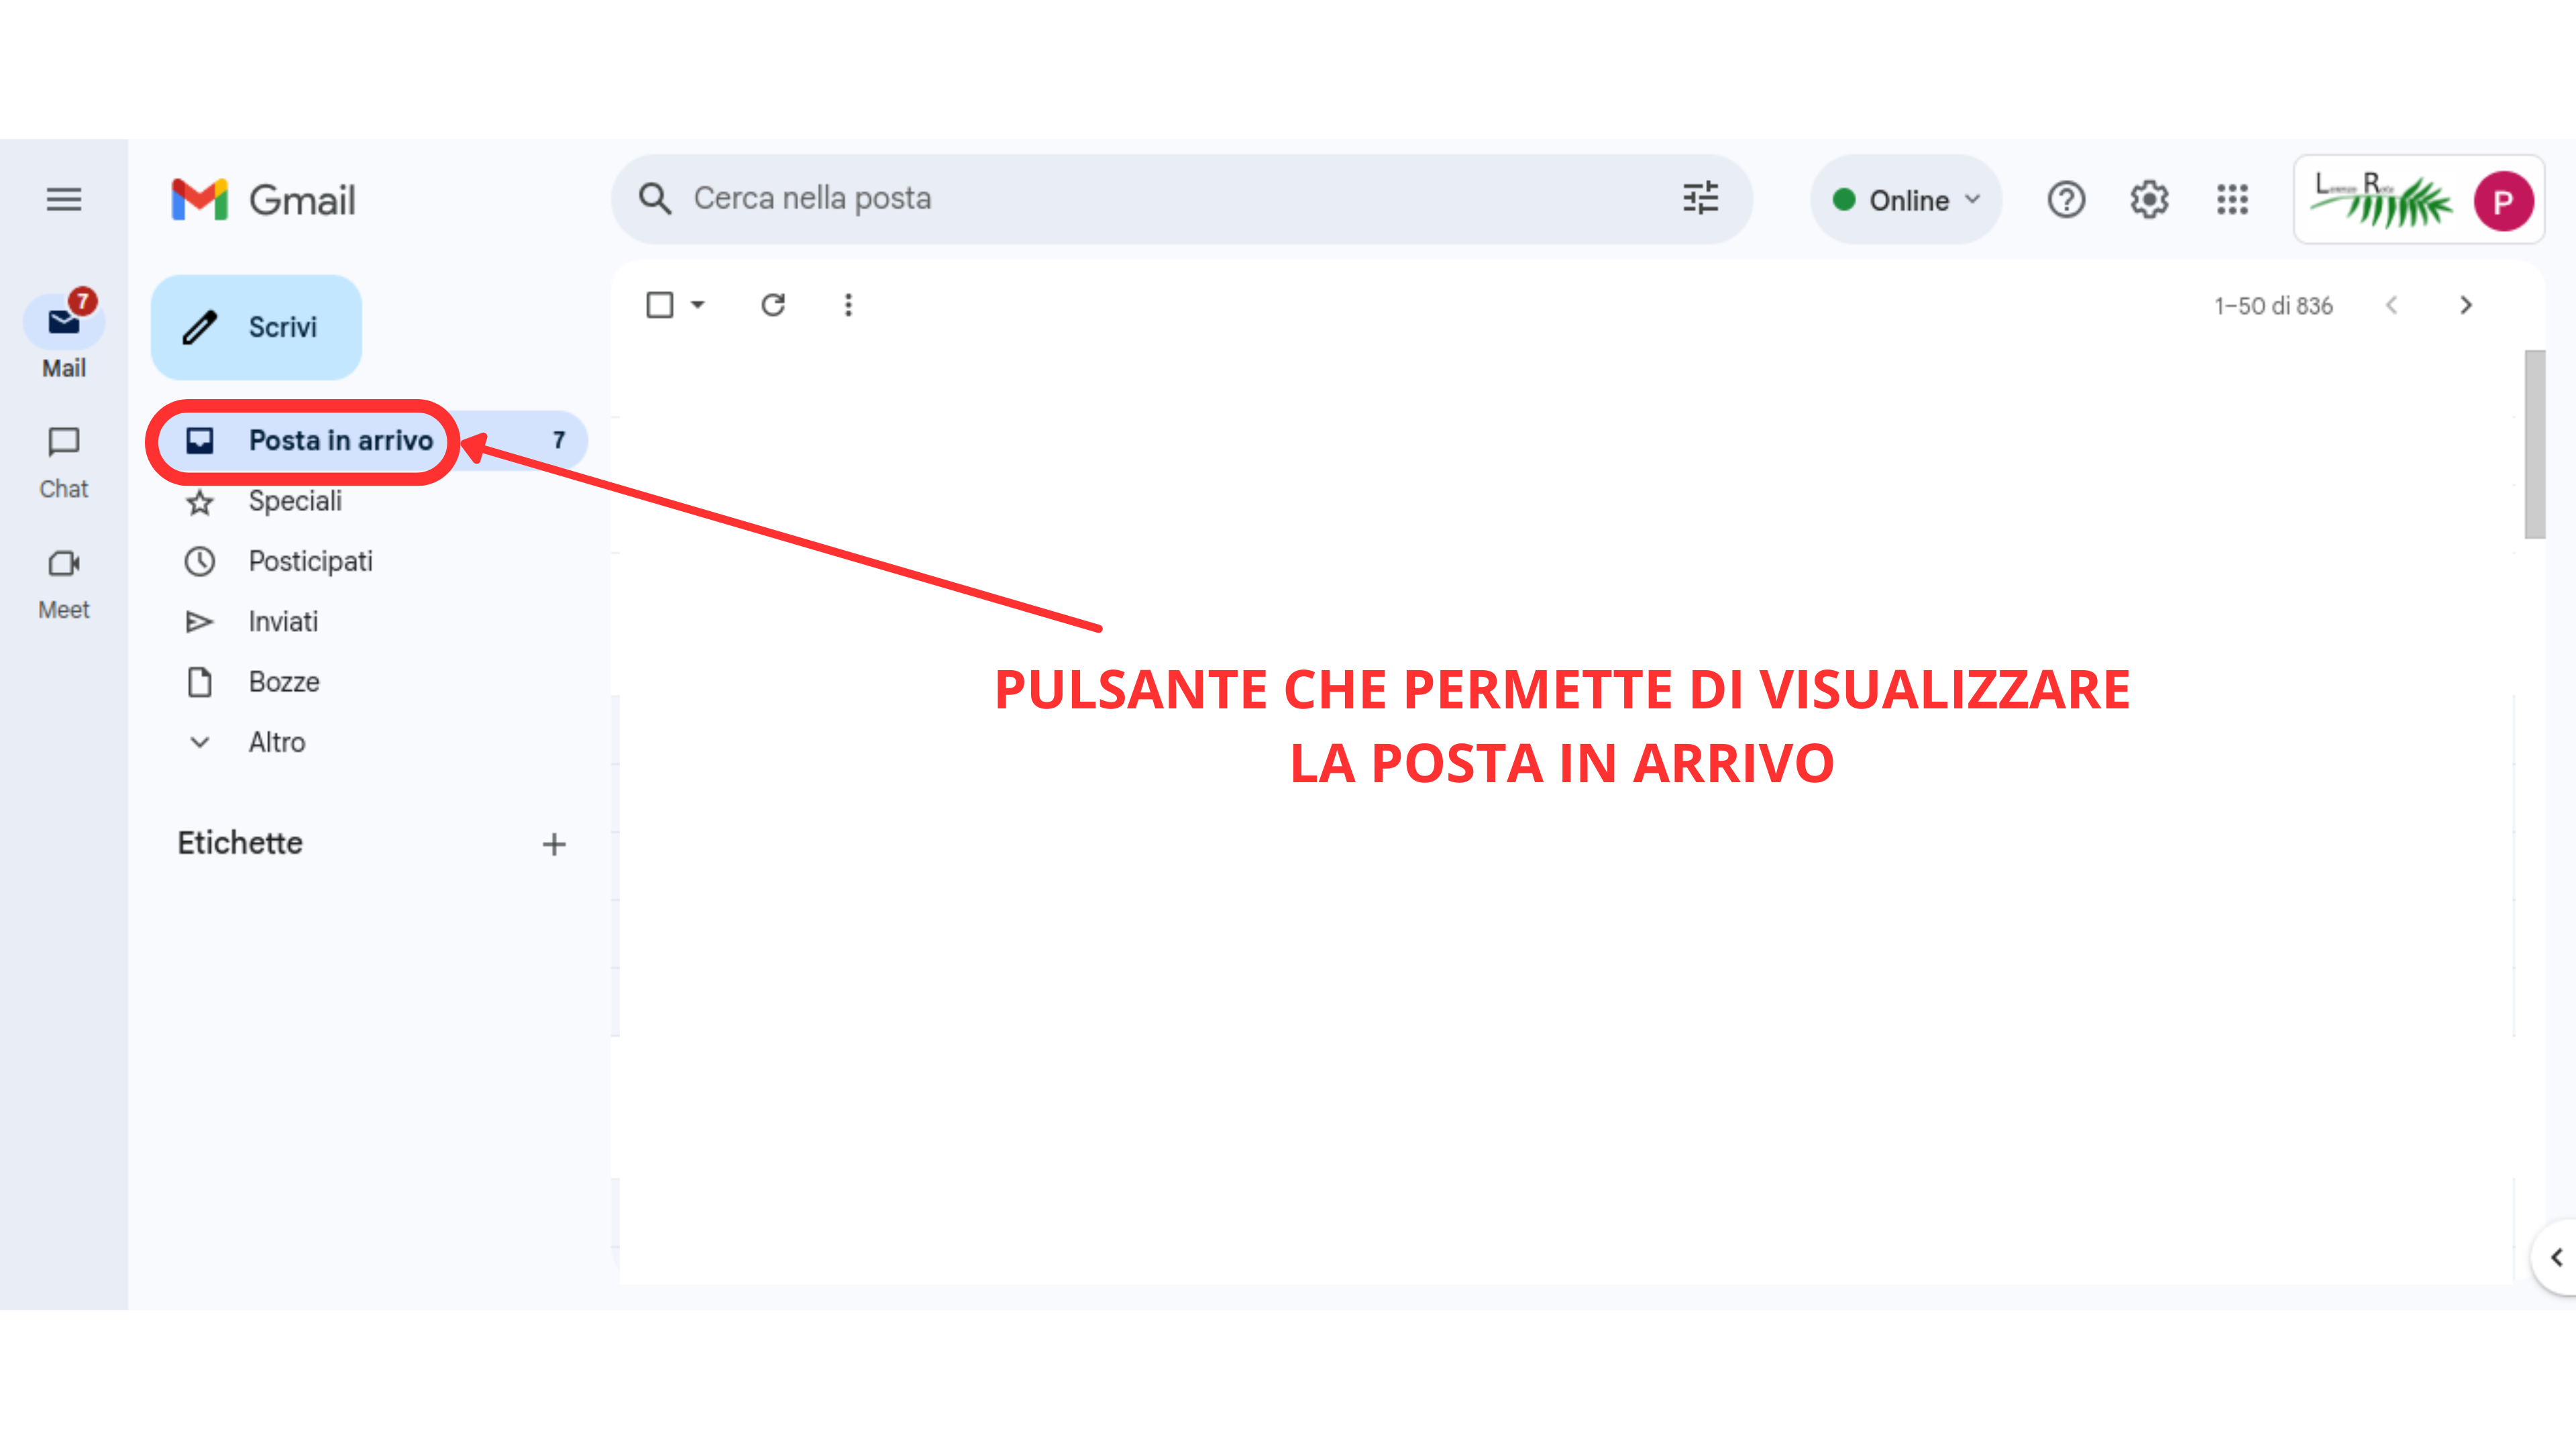
\includegraphics[width=\linewidth]{img/mail1.png}
        \caption{{screenshot della homepage di \href{https://mail.google.com/}{Google Mail}}, modificato con \href{https://www.canva.com}{Canva}}
    \end{figure}}
    \only<2>{\begin{figure}
        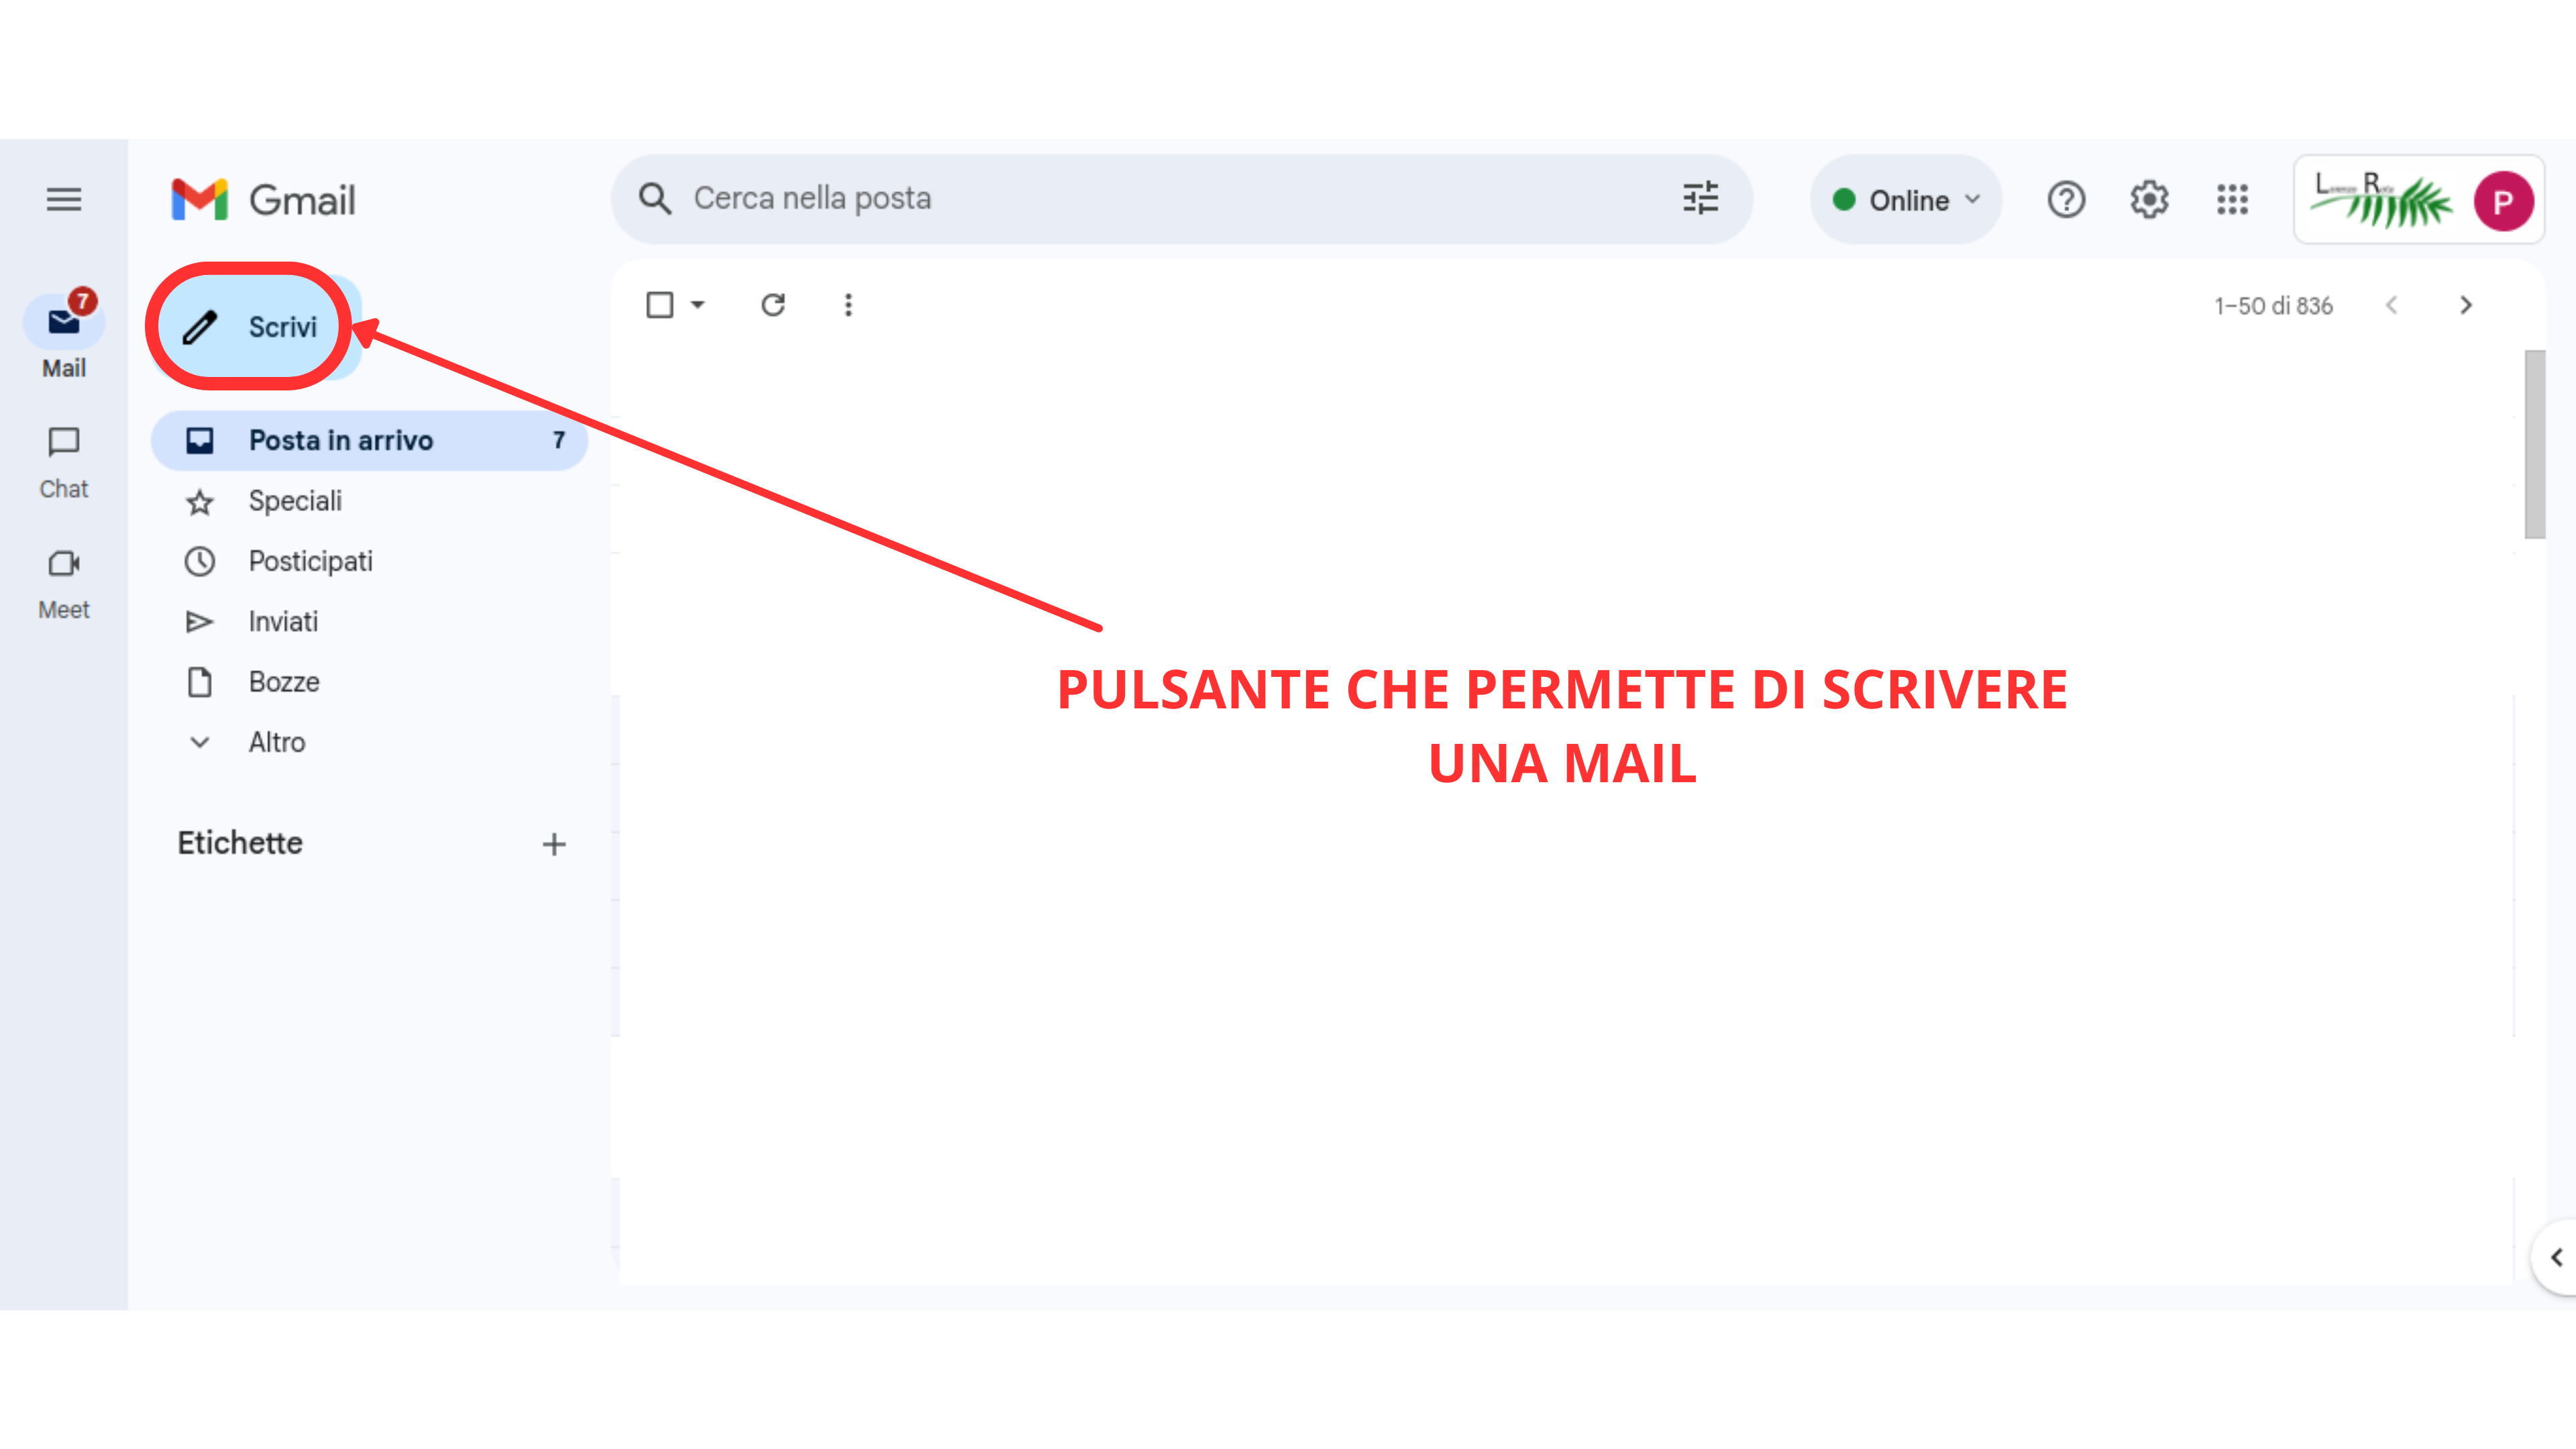
\includegraphics[width=\linewidth]{img/mail2.png}
        \caption{{screenshot della homepage di \href{https://mail.google.com/}{Google Mail}}, modificato con \href{https://www.canva.com}{Canva}}
    \end{figure}}
    \only<3>{\begin{figure}
        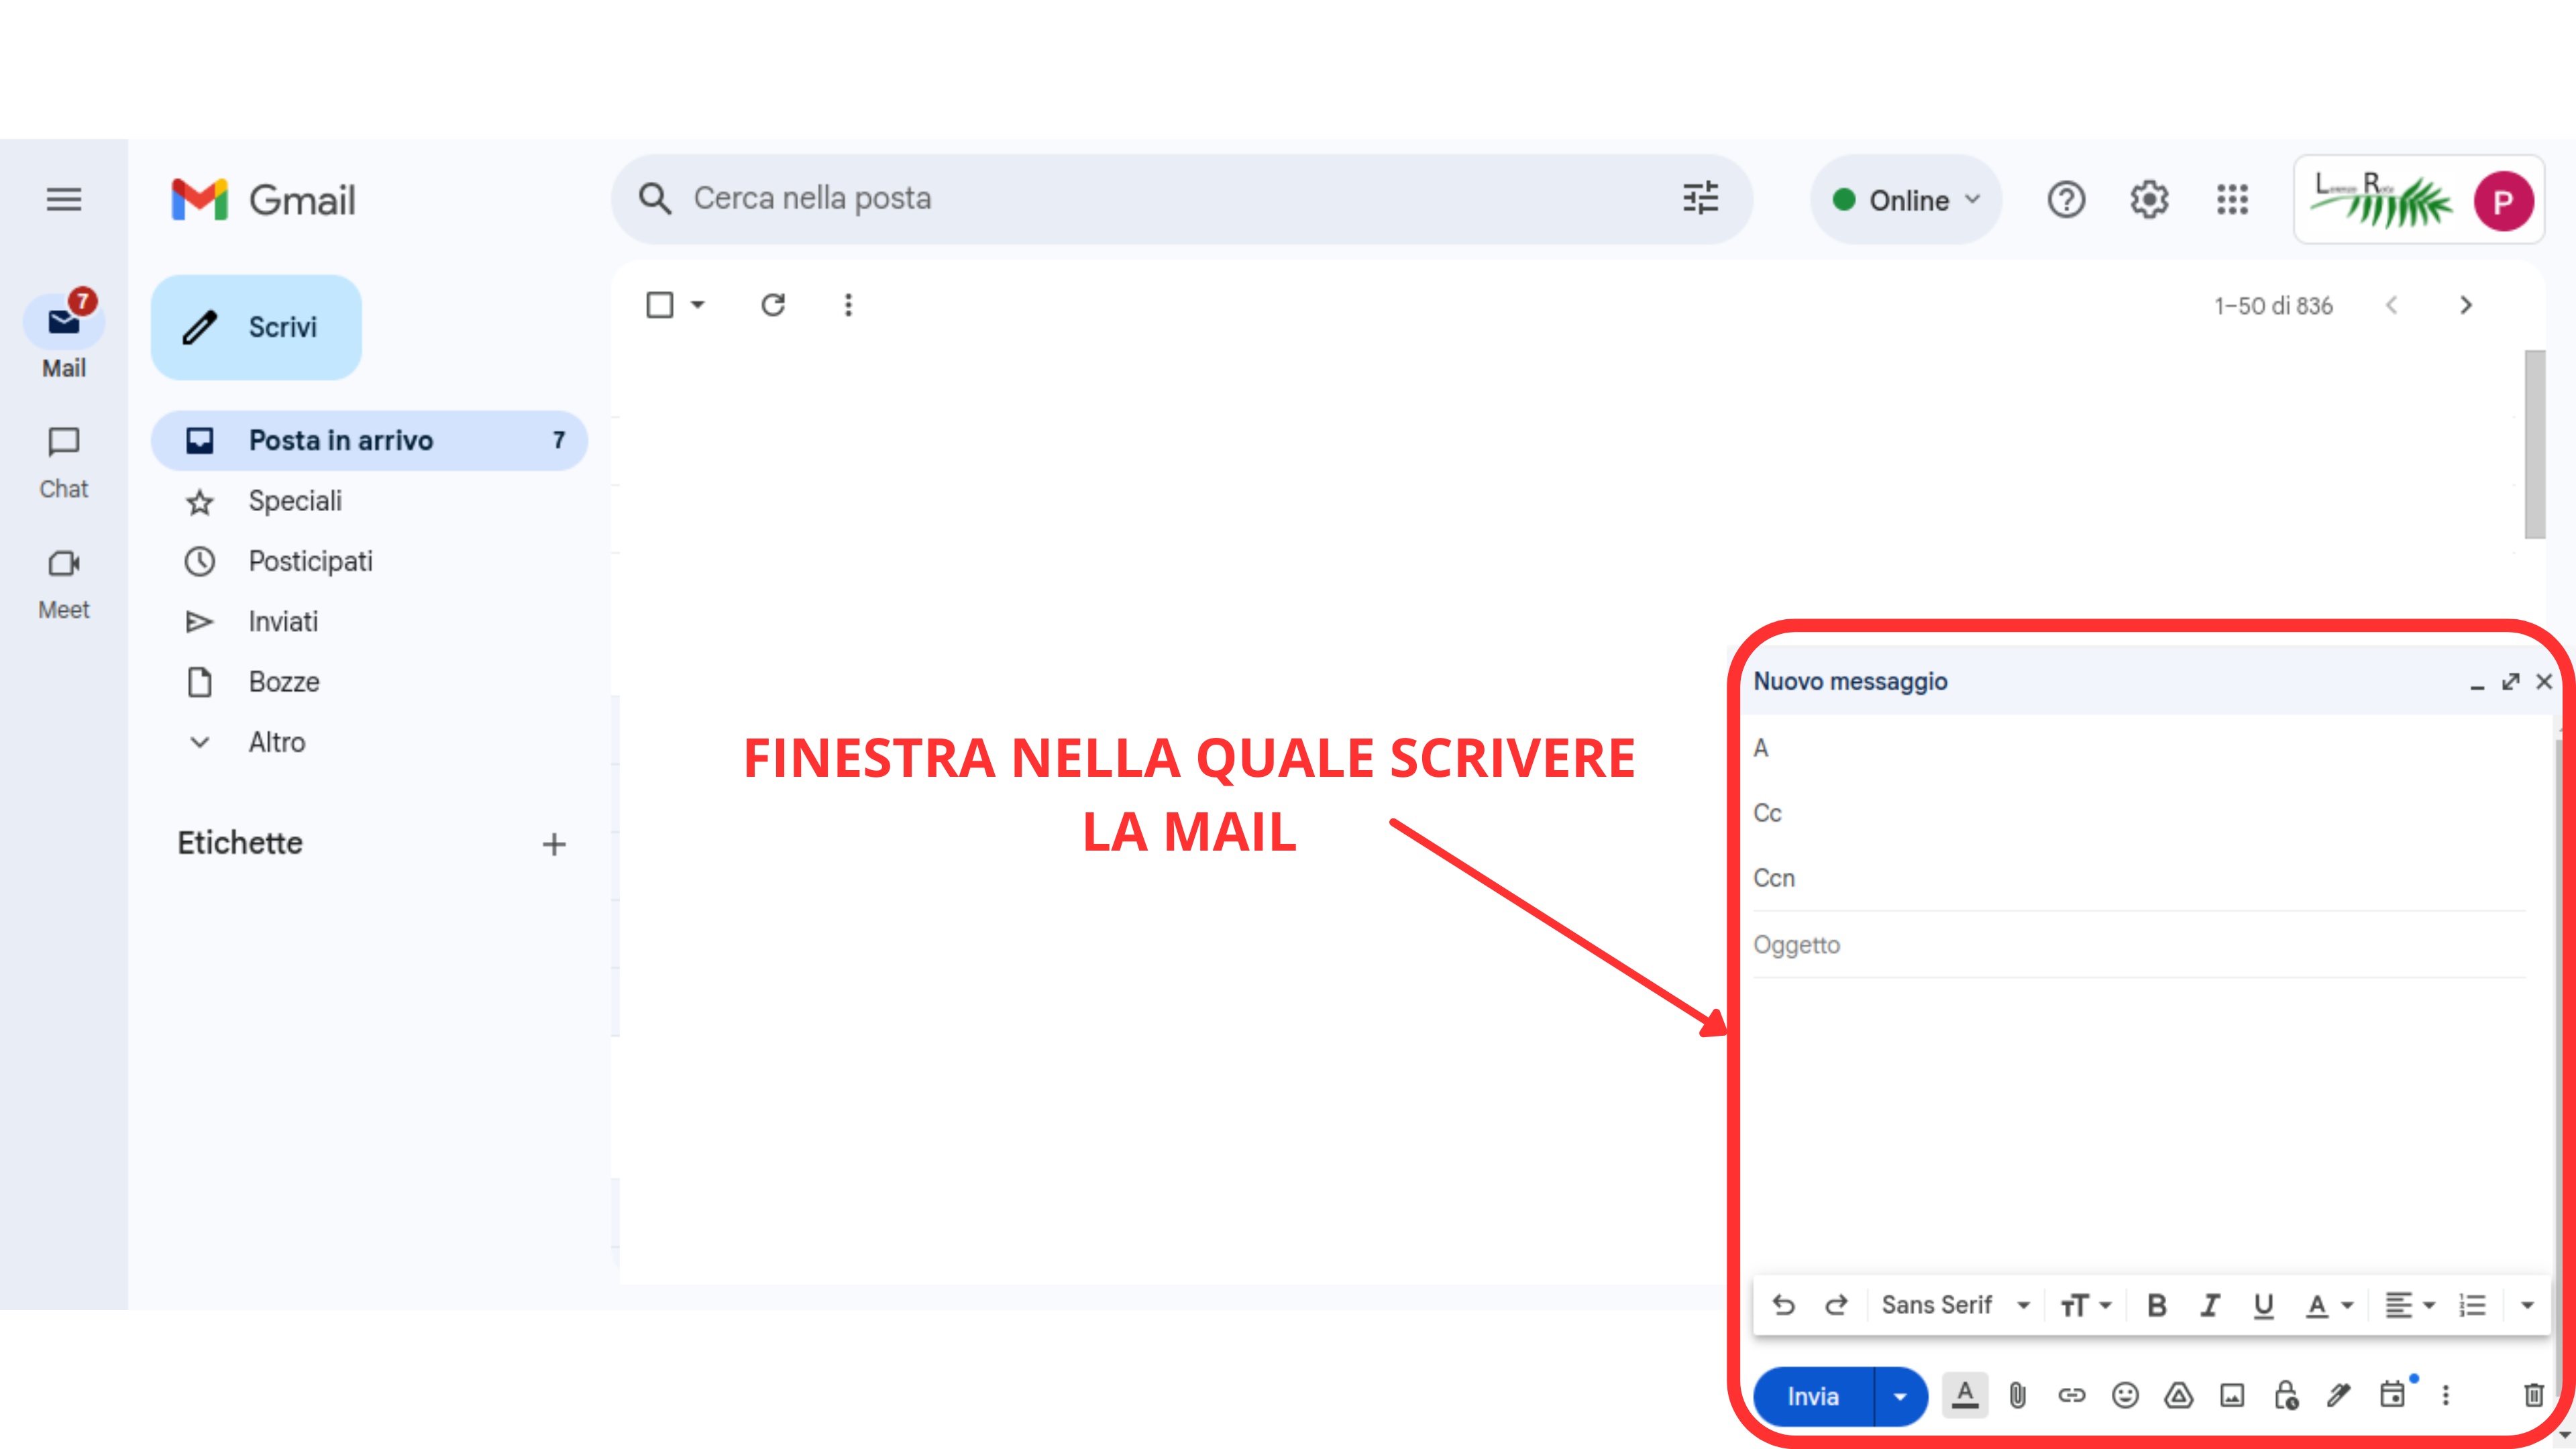
\includegraphics[width=\linewidth]{img/mail3.png}
        \caption{{screenshot della homepage di \href{https://mail.google.com/}{Google Mail}}, modificato con \href{https://www.canva.com}{Canva}}
    \end{figure}}
    \only<4>{\begin{figure}
        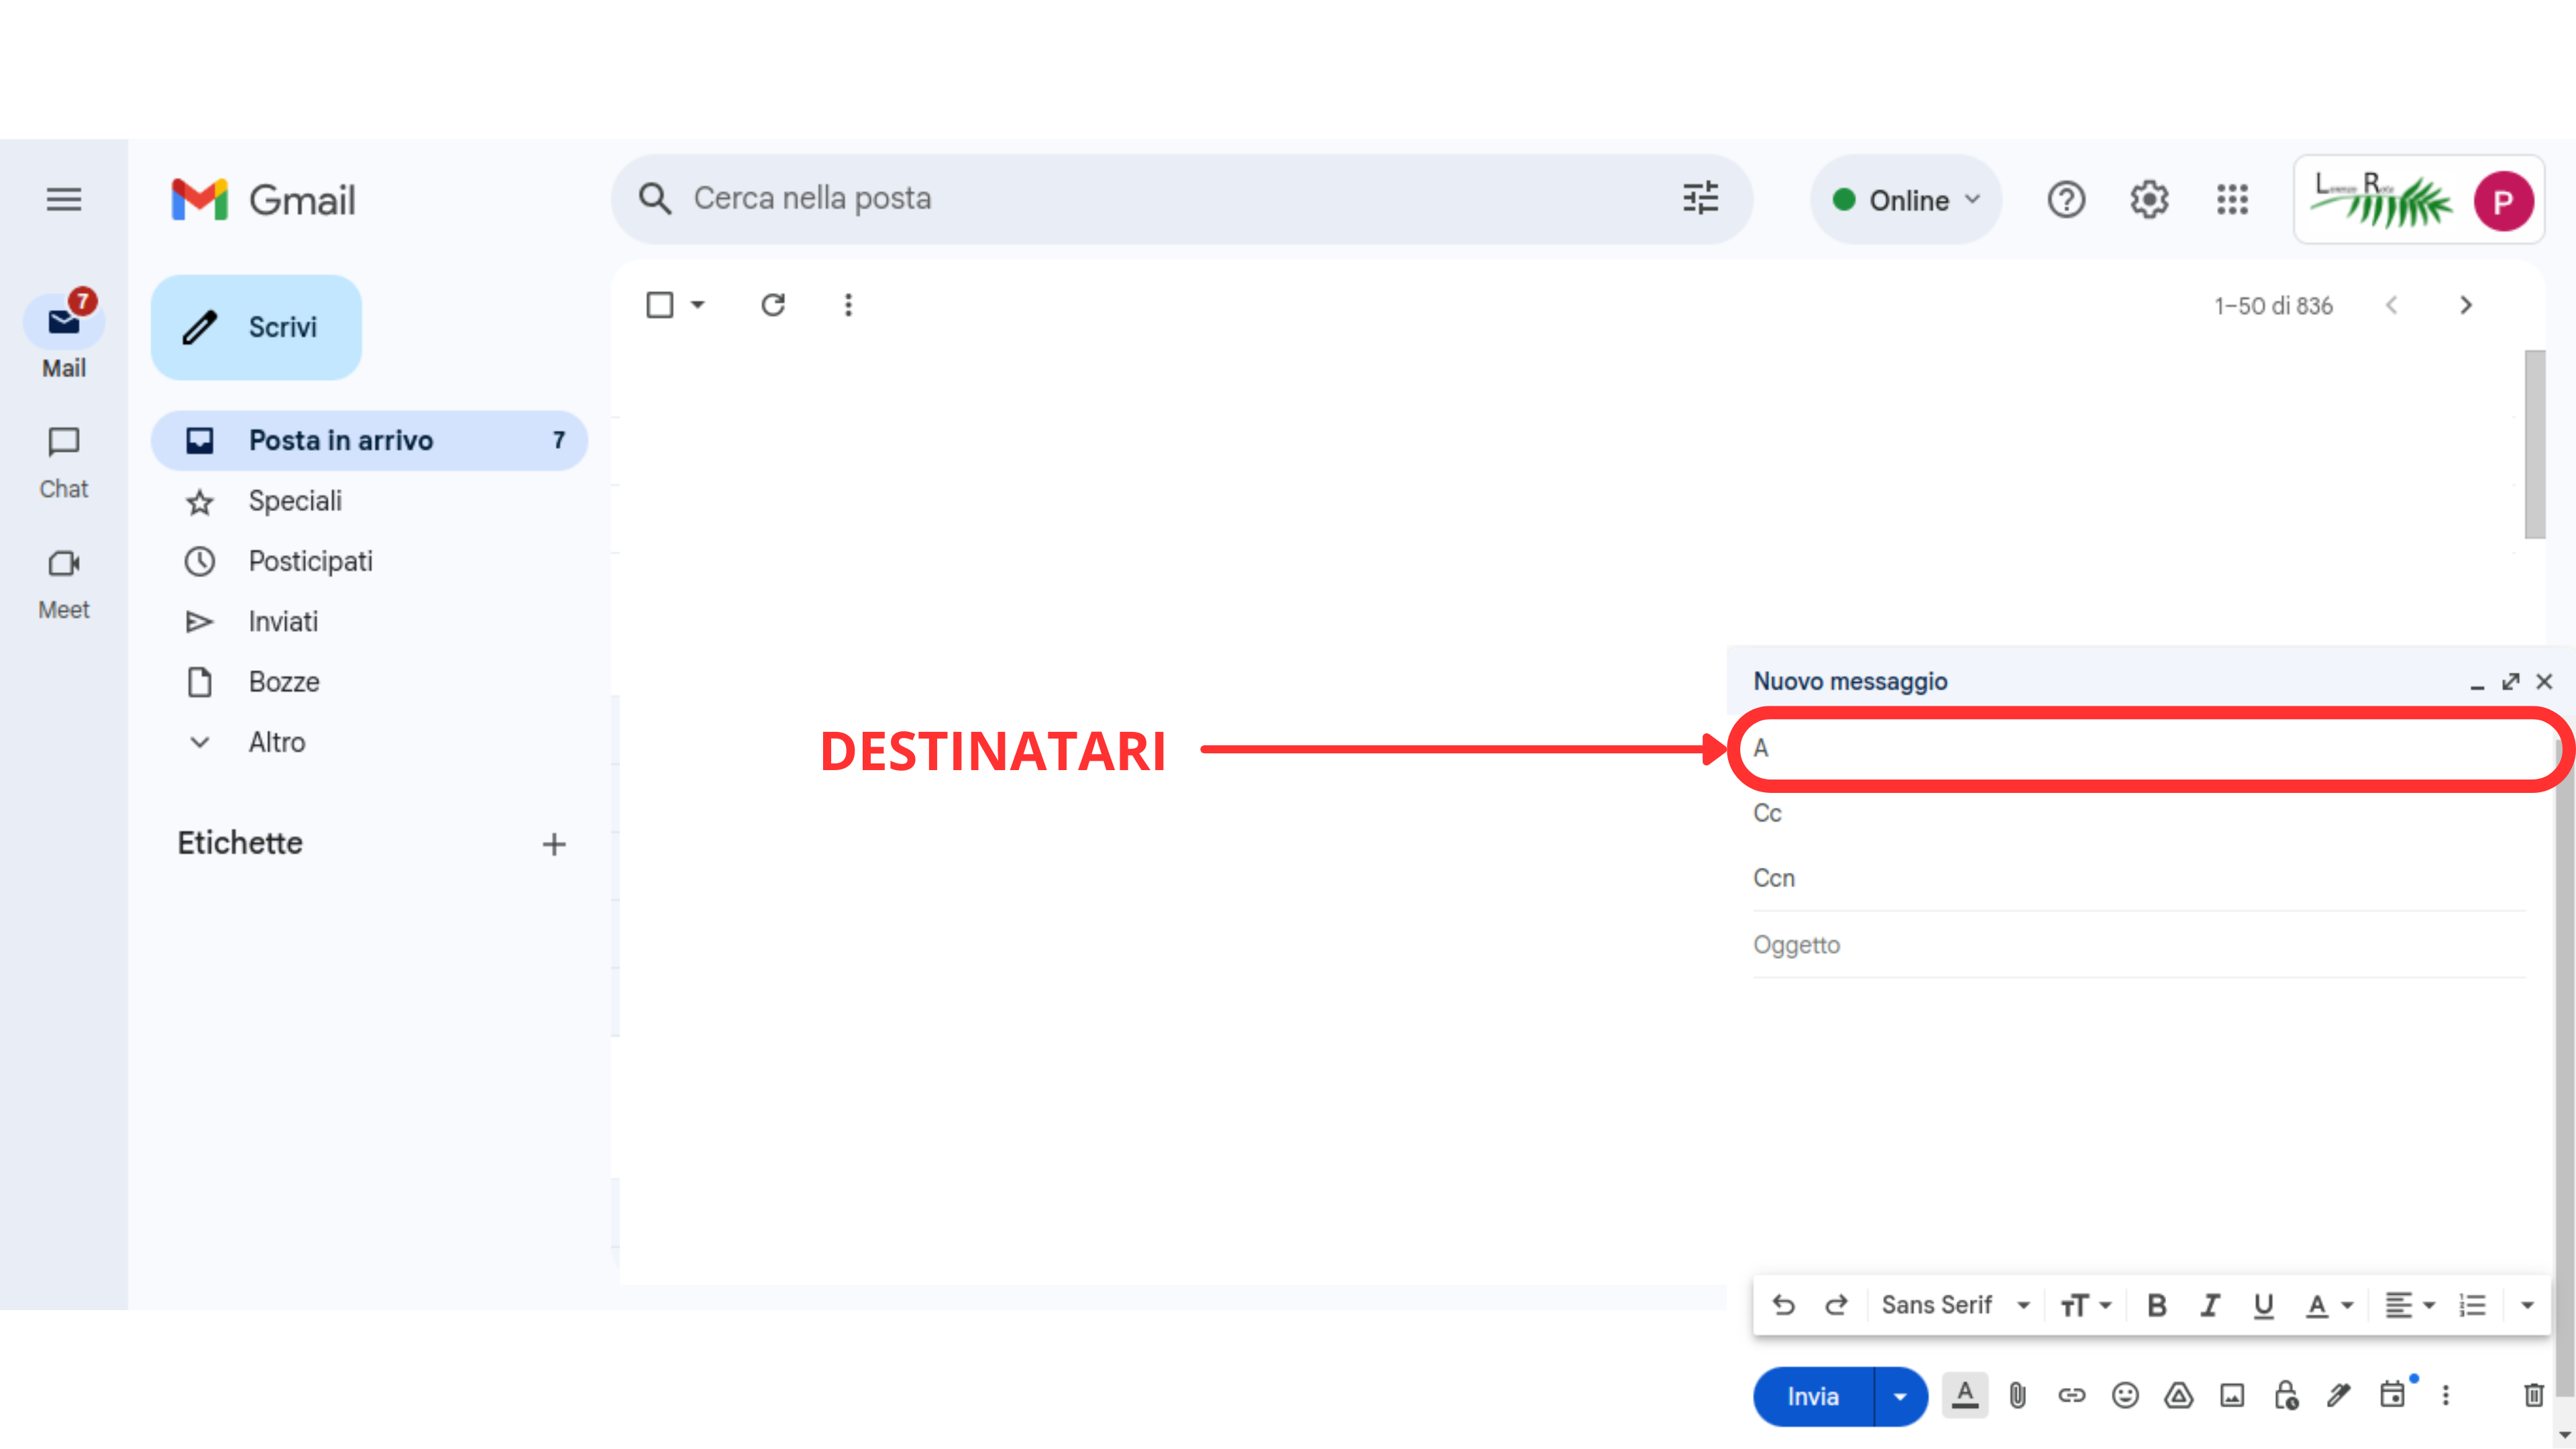
\includegraphics[width=\linewidth]{img/mail4.png}
        \caption{{screenshot della homepage di \href{https://mail.google.com/}{Google Mail}}, modificato con \href{https://www.canva.com}{Canva}}
    \end{figure}}
    \only<5>{\begin{figure}
        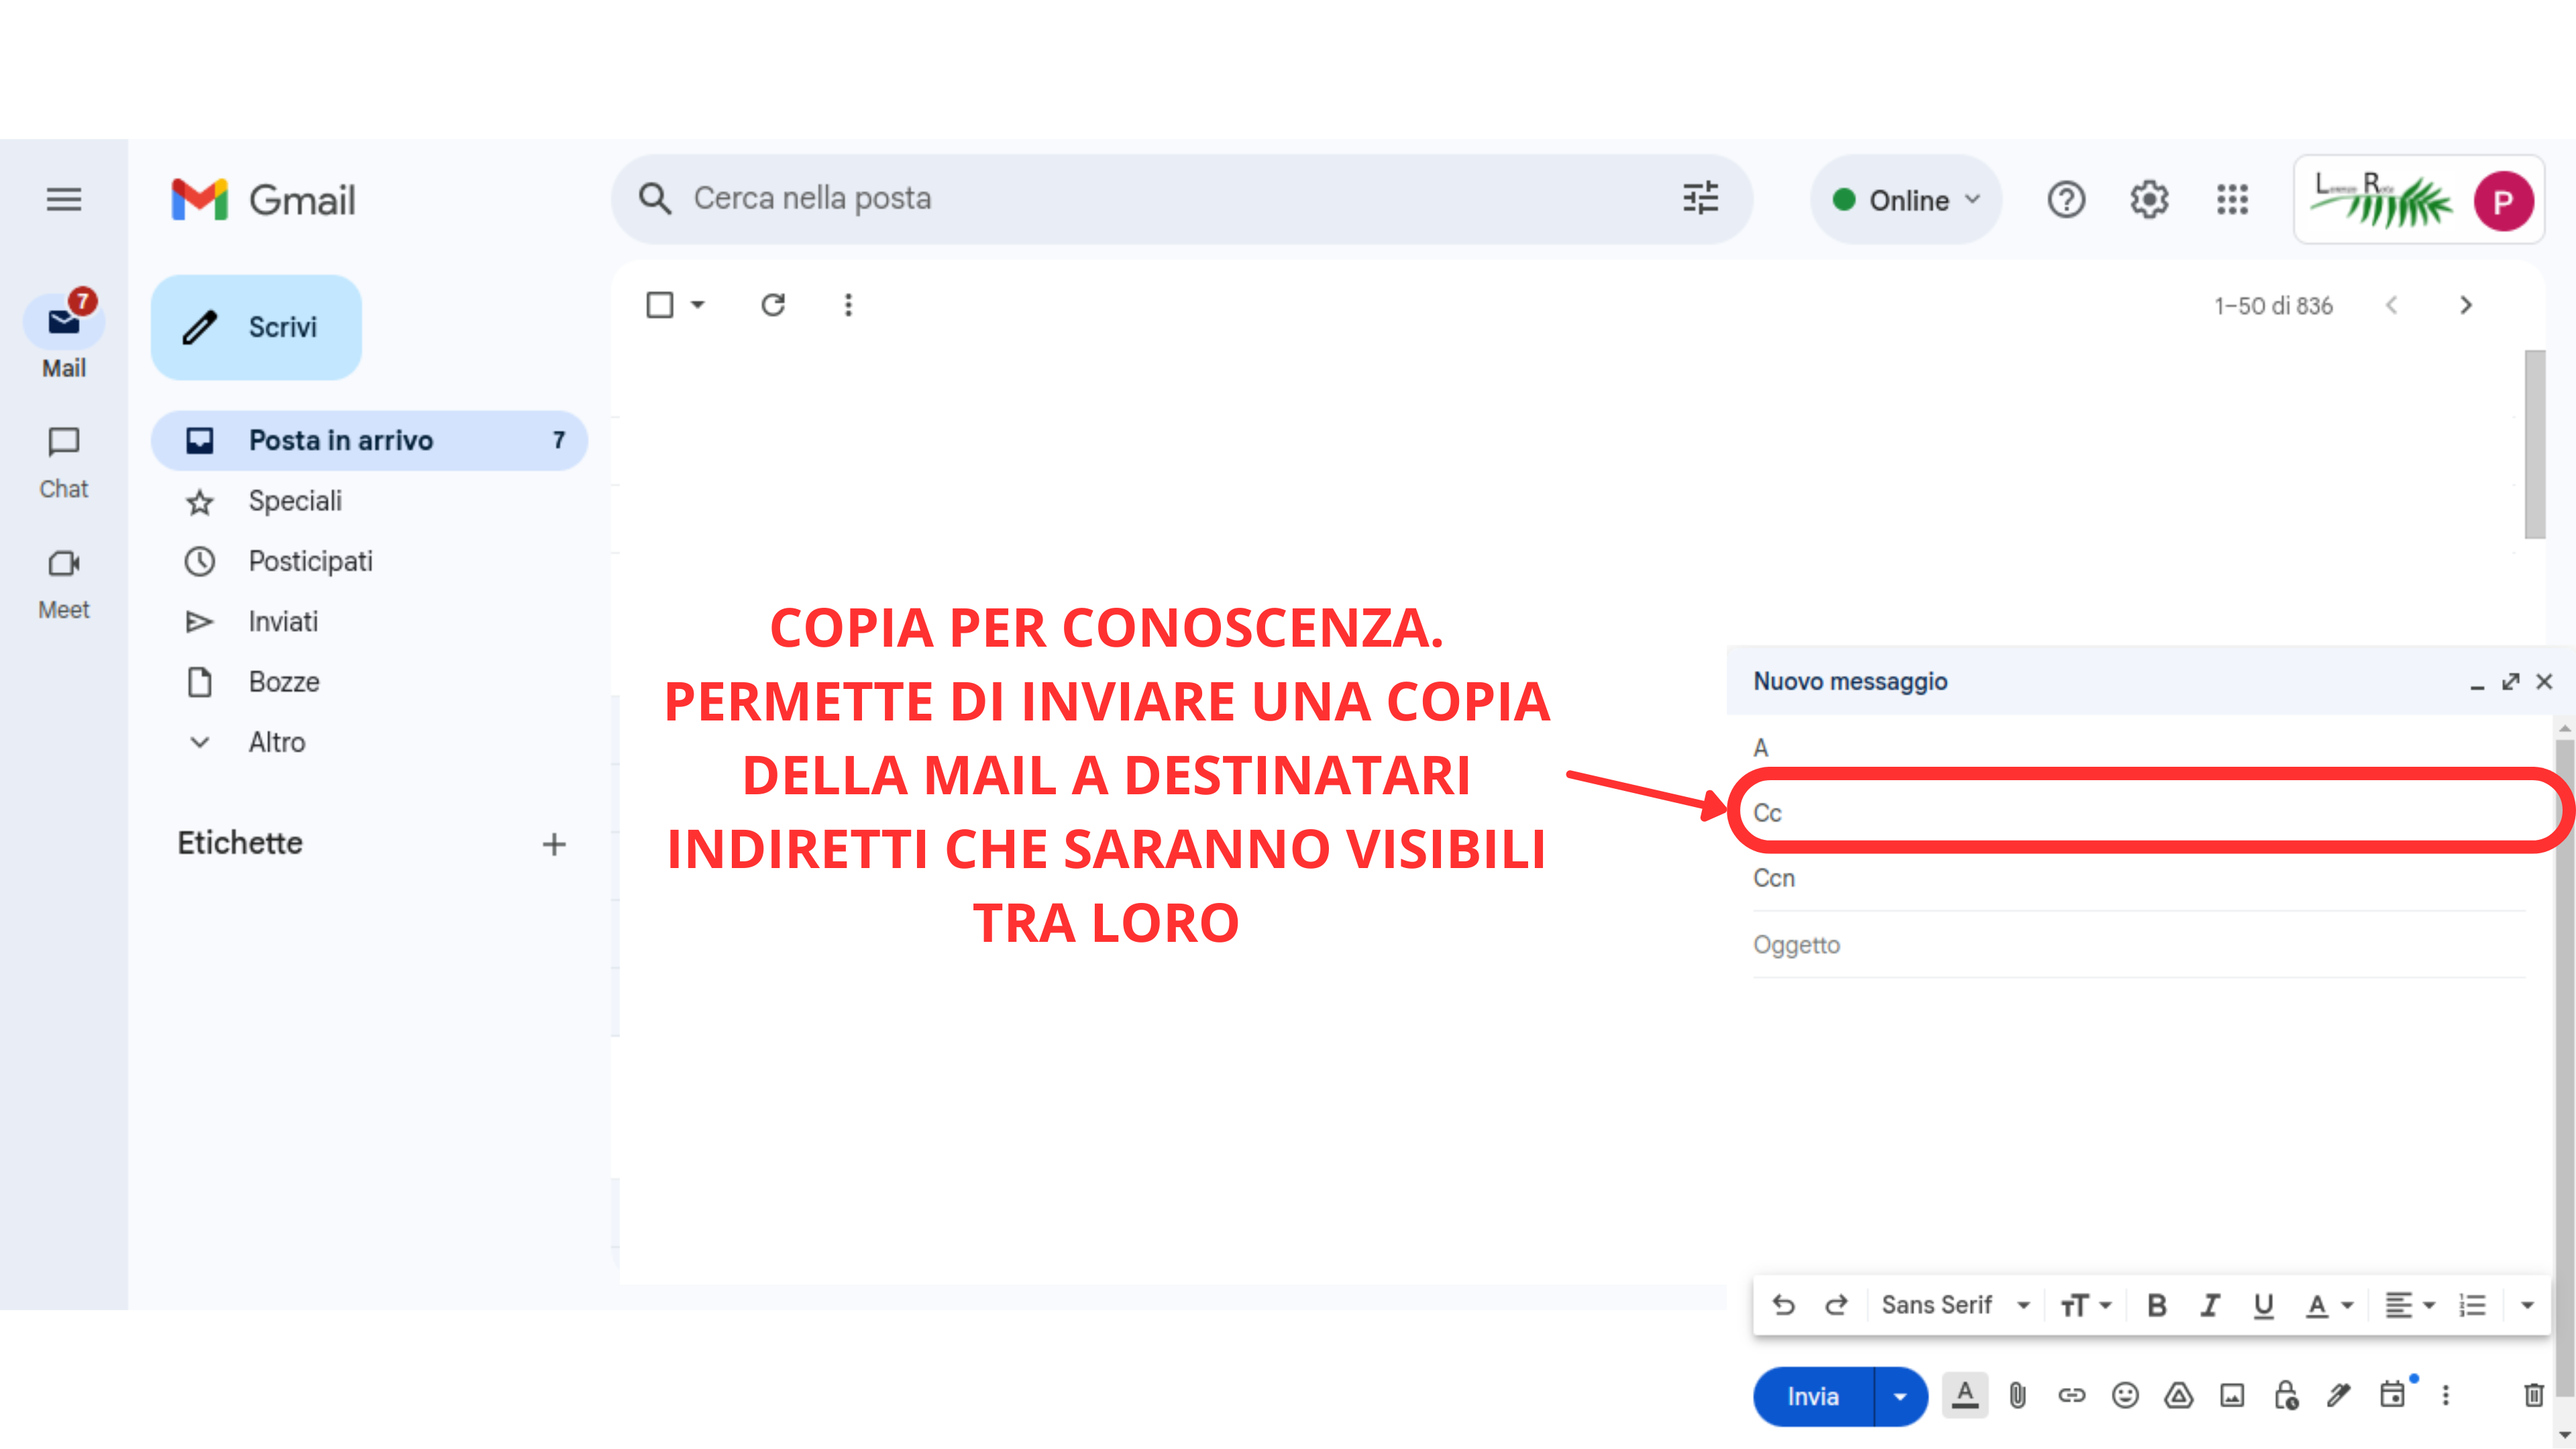
\includegraphics[width=\linewidth]{img/mail5.png}
        \caption{{screenshot della homepage di \href{https://mail.google.com/}{Google Mail}}, modificato con \href{https://www.canva.com}{Canva}}
    \end{figure}}
    \only<6>{\begin{figure}
        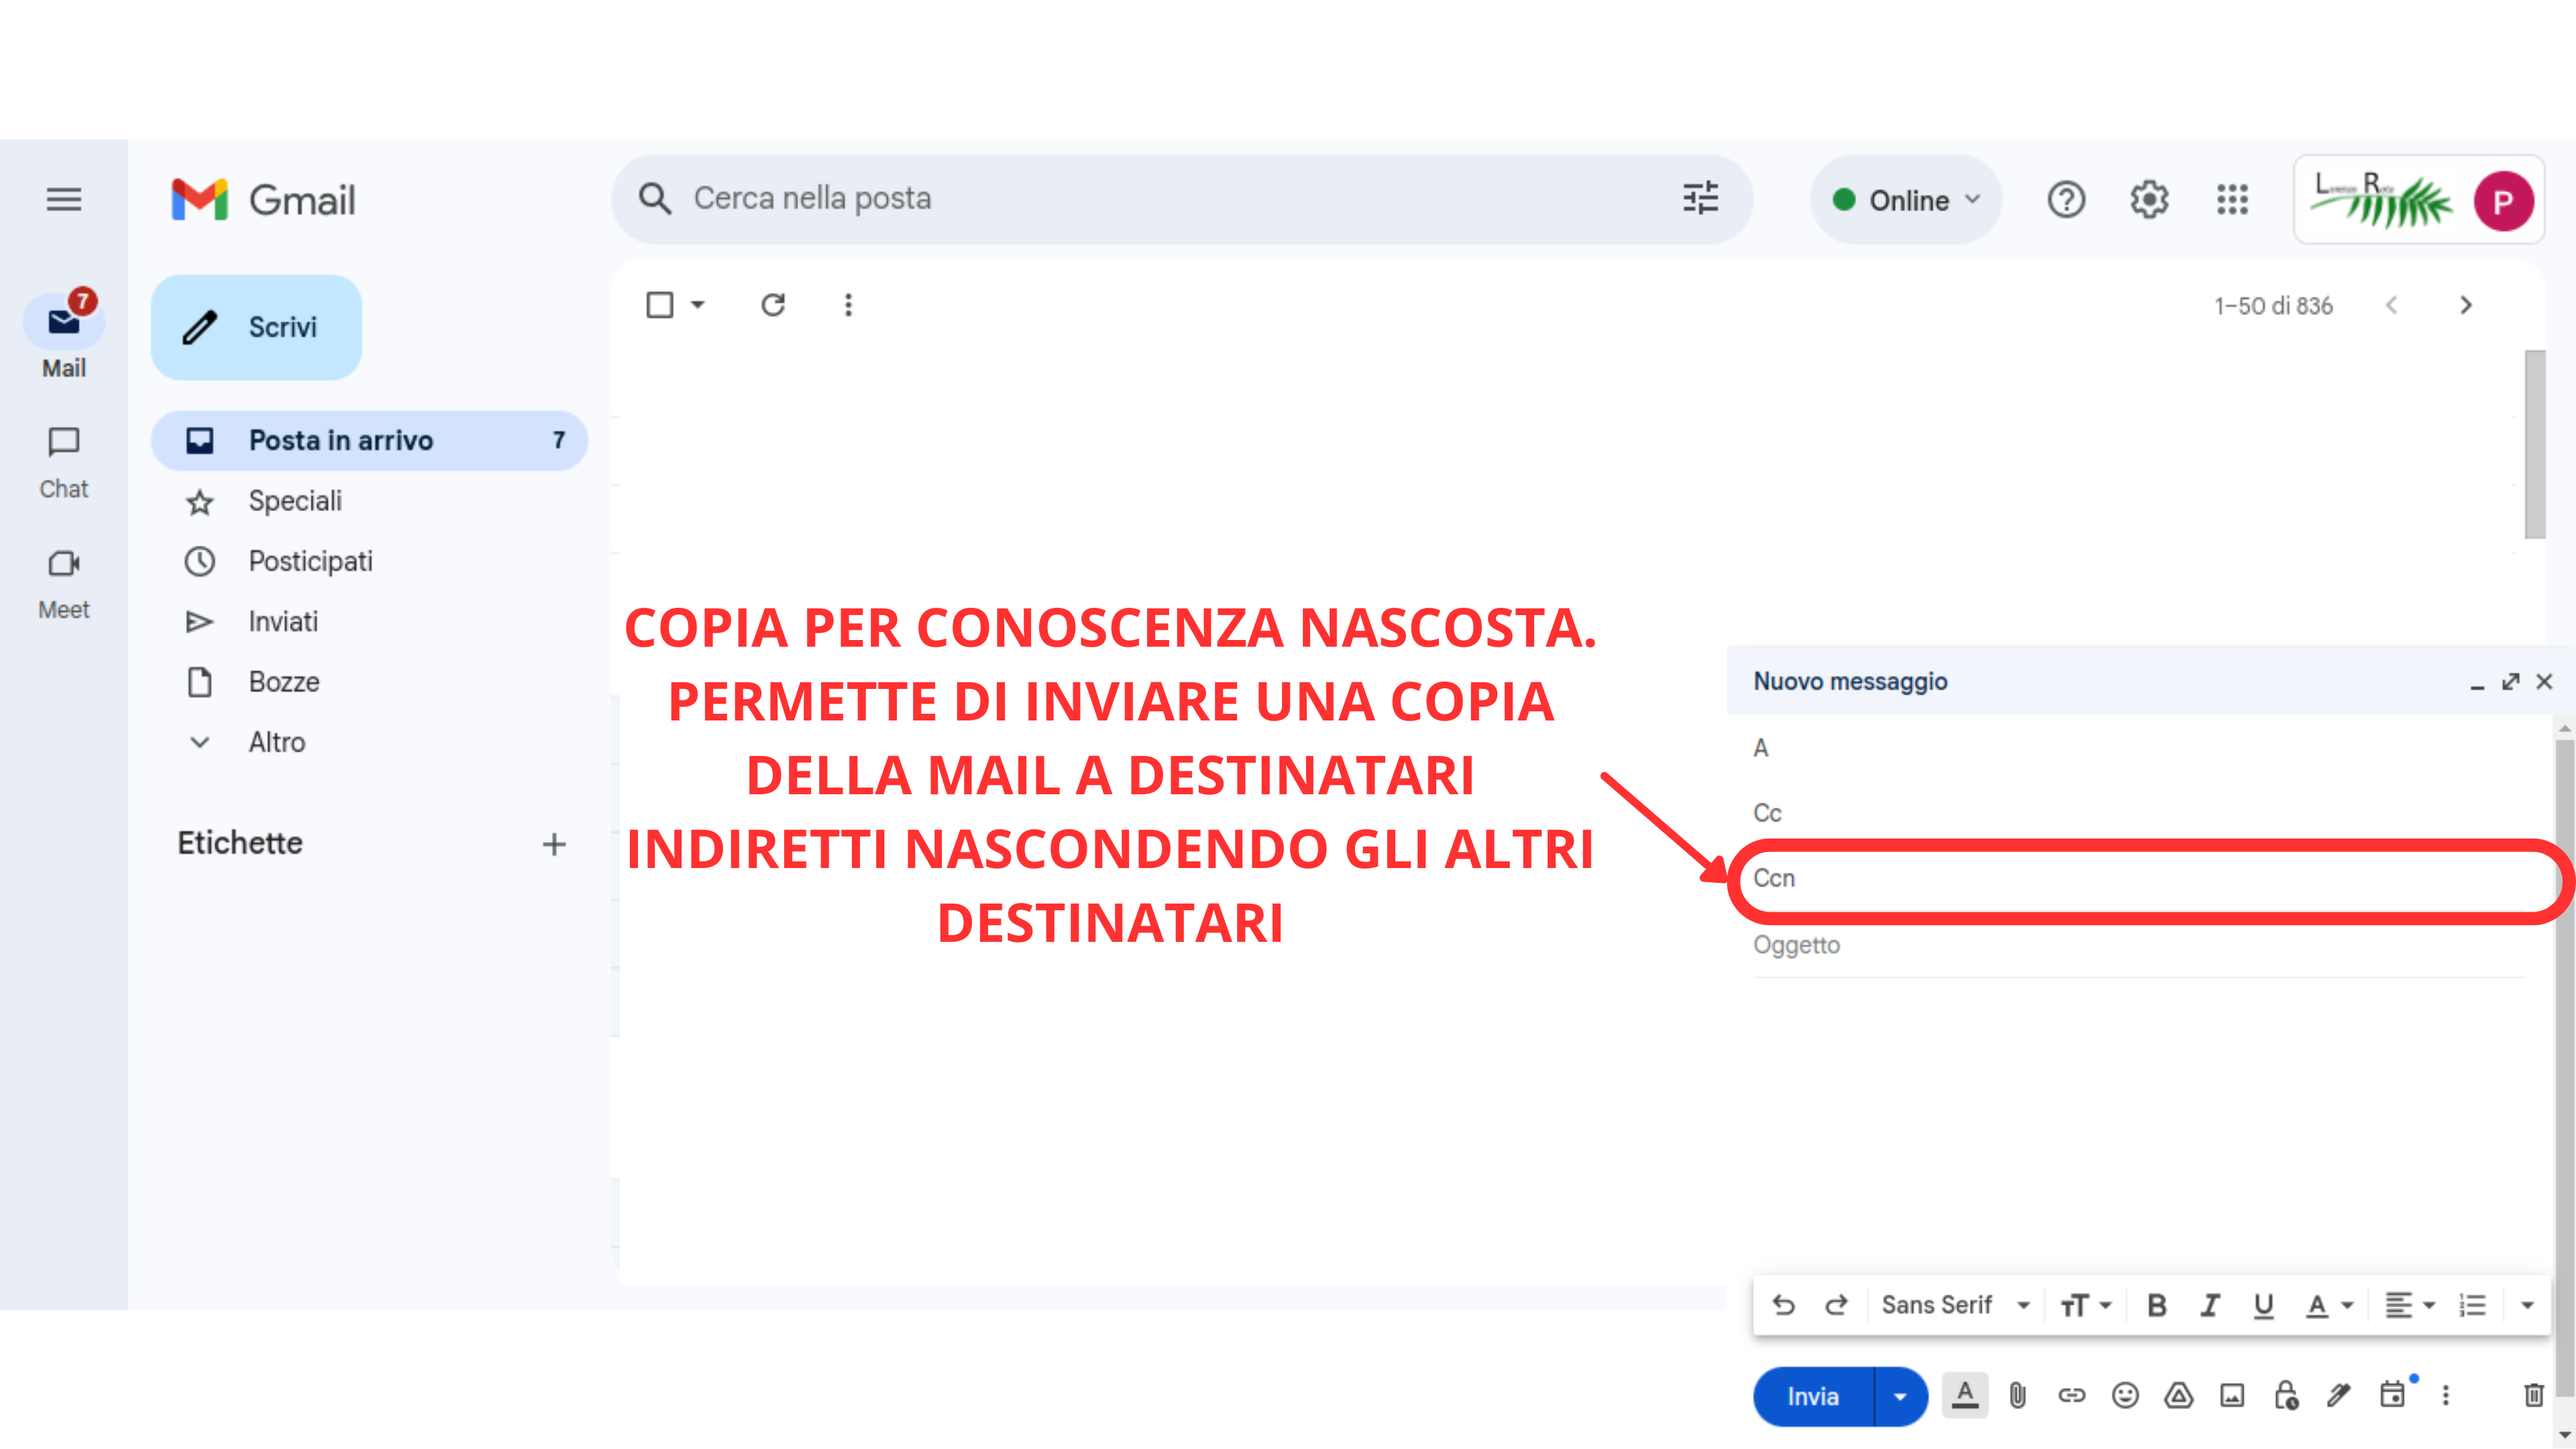
\includegraphics[width=\linewidth]{img/mail6.png}
        \caption{{screenshot della homepage di \href{https://mail.google.com/}{Google Mail}}, modificato con \href{https://www.canva.com}{Canva}}
    \end{figure}}
    \only<7>{\begin{figure}
        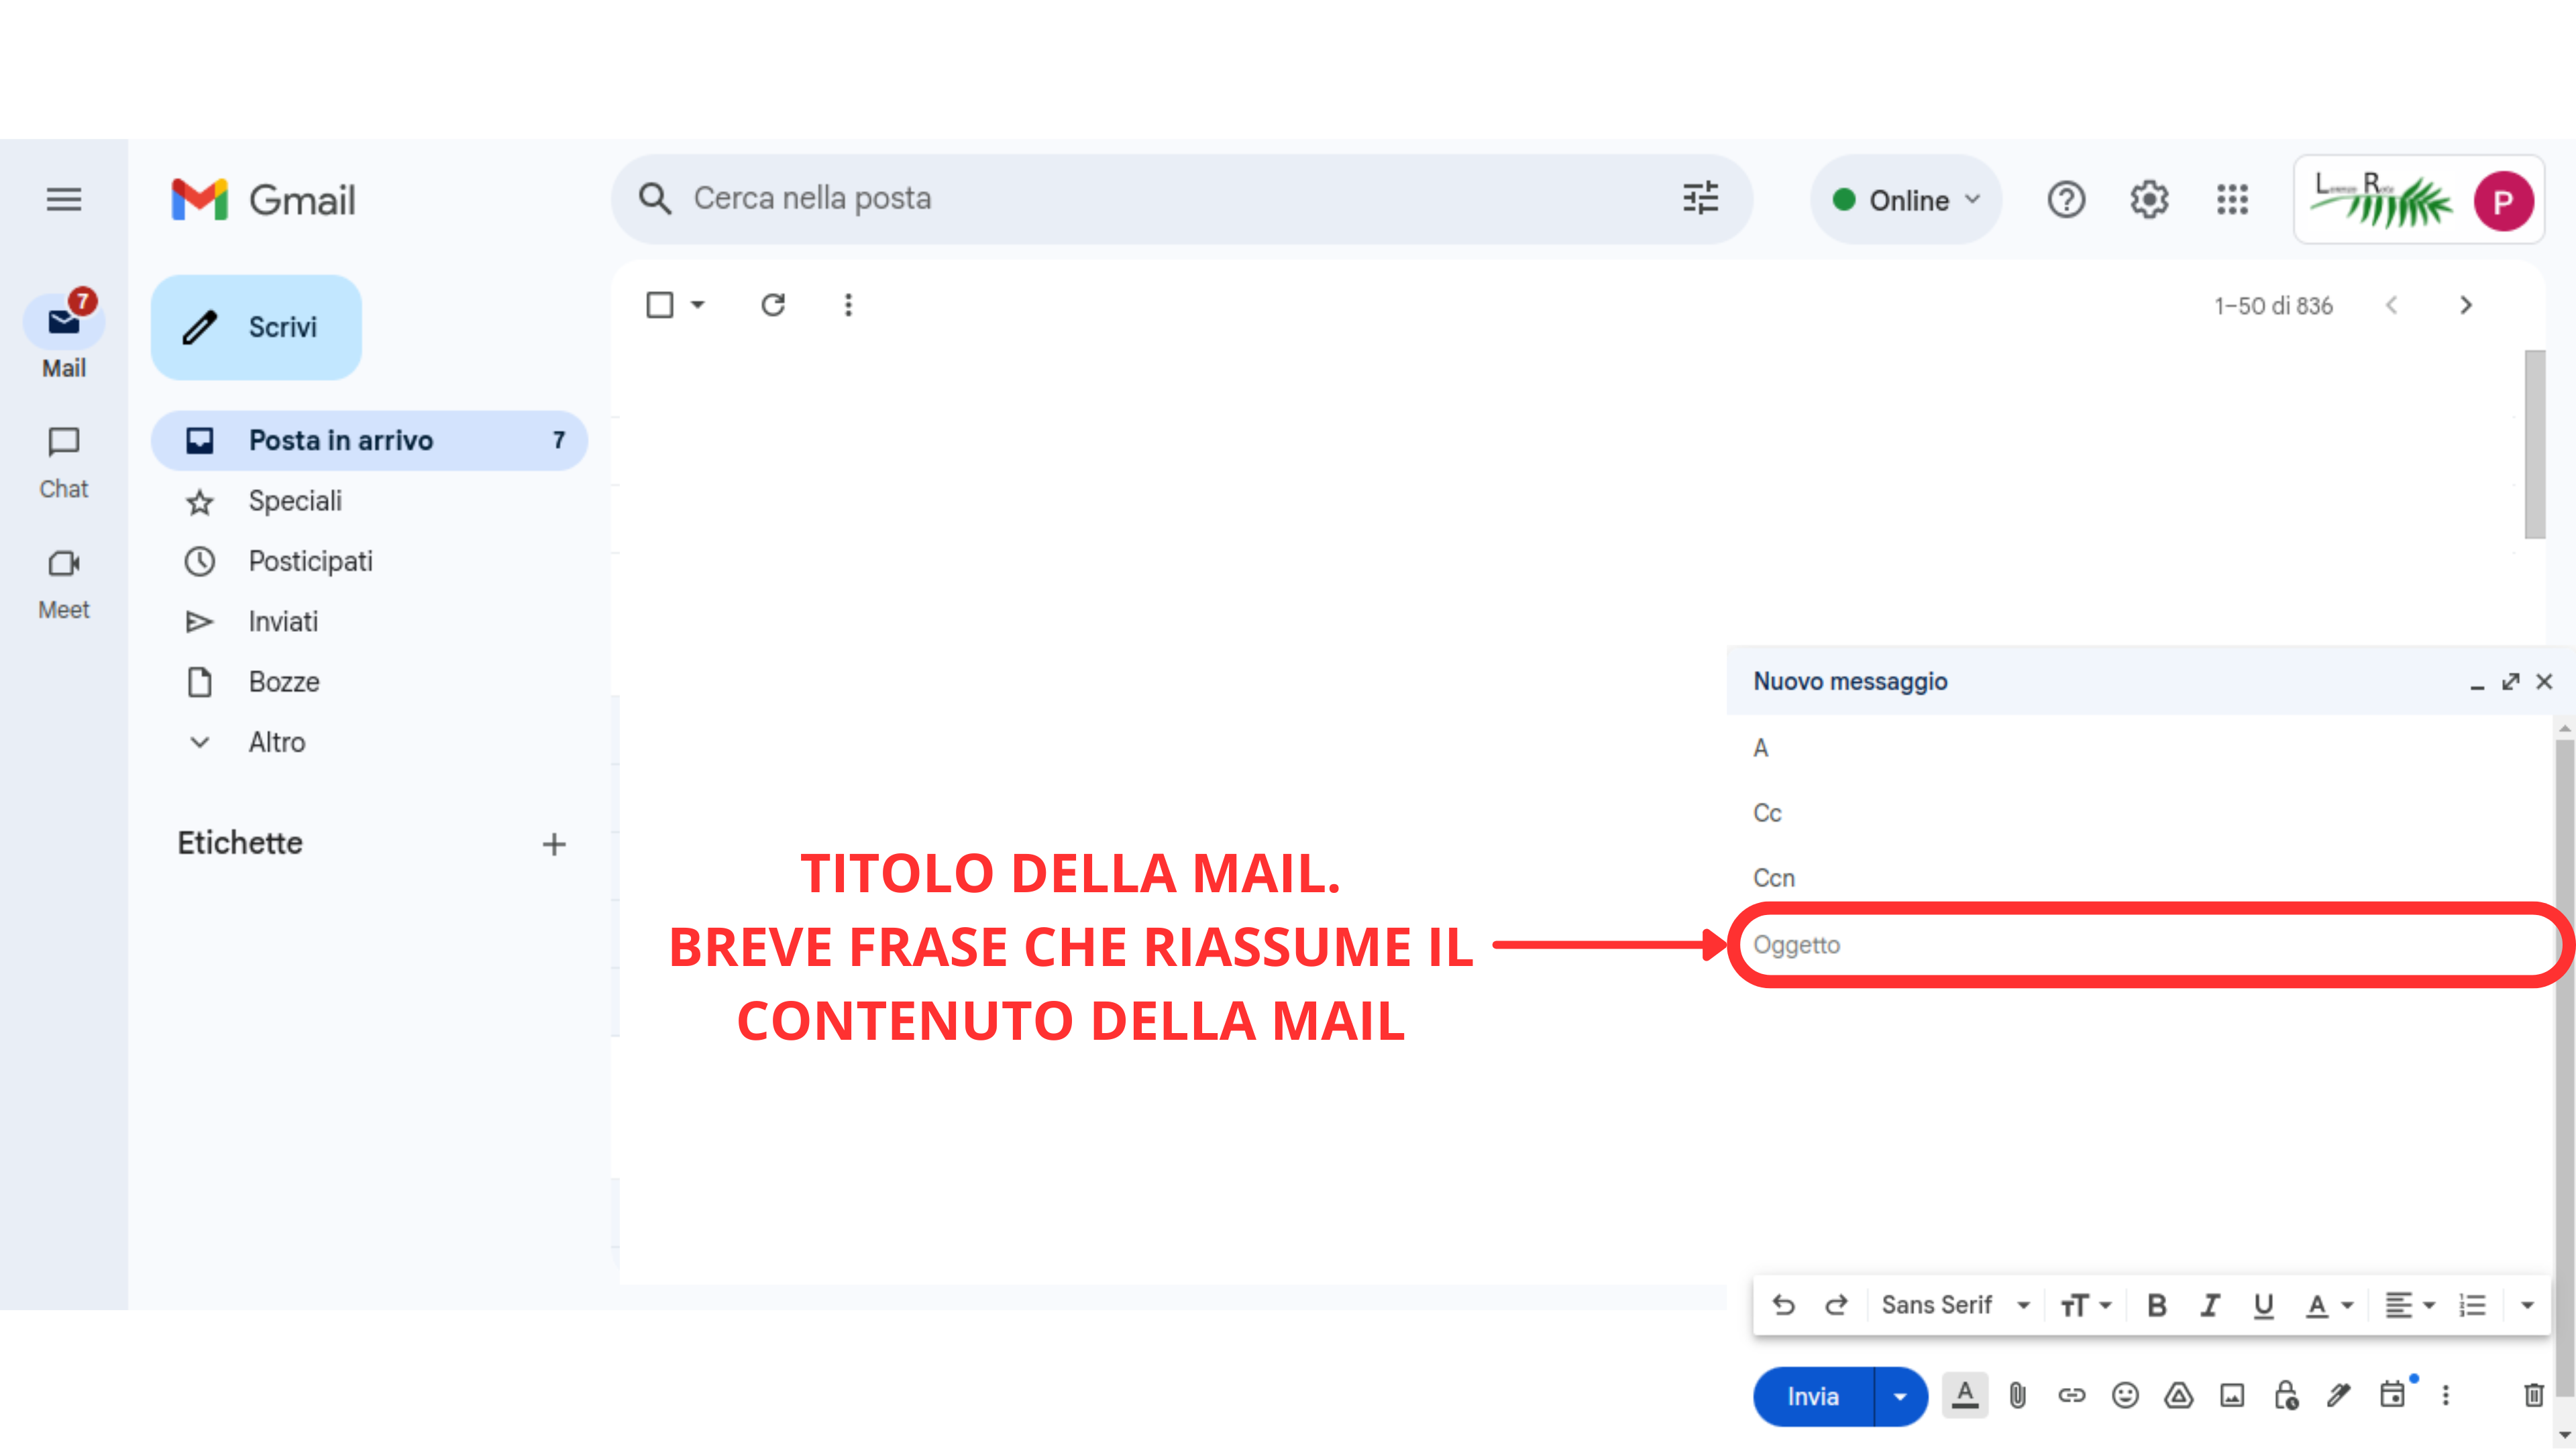
\includegraphics[width=\linewidth]{img/mail7.png}
        \caption{{screenshot della homepage di \href{https://mail.google.com/}{Google Mail}}, modificato con \href{https://www.canva.com}{Canva}}
    \end{figure}}
    \only<8>{\begin{figure}
        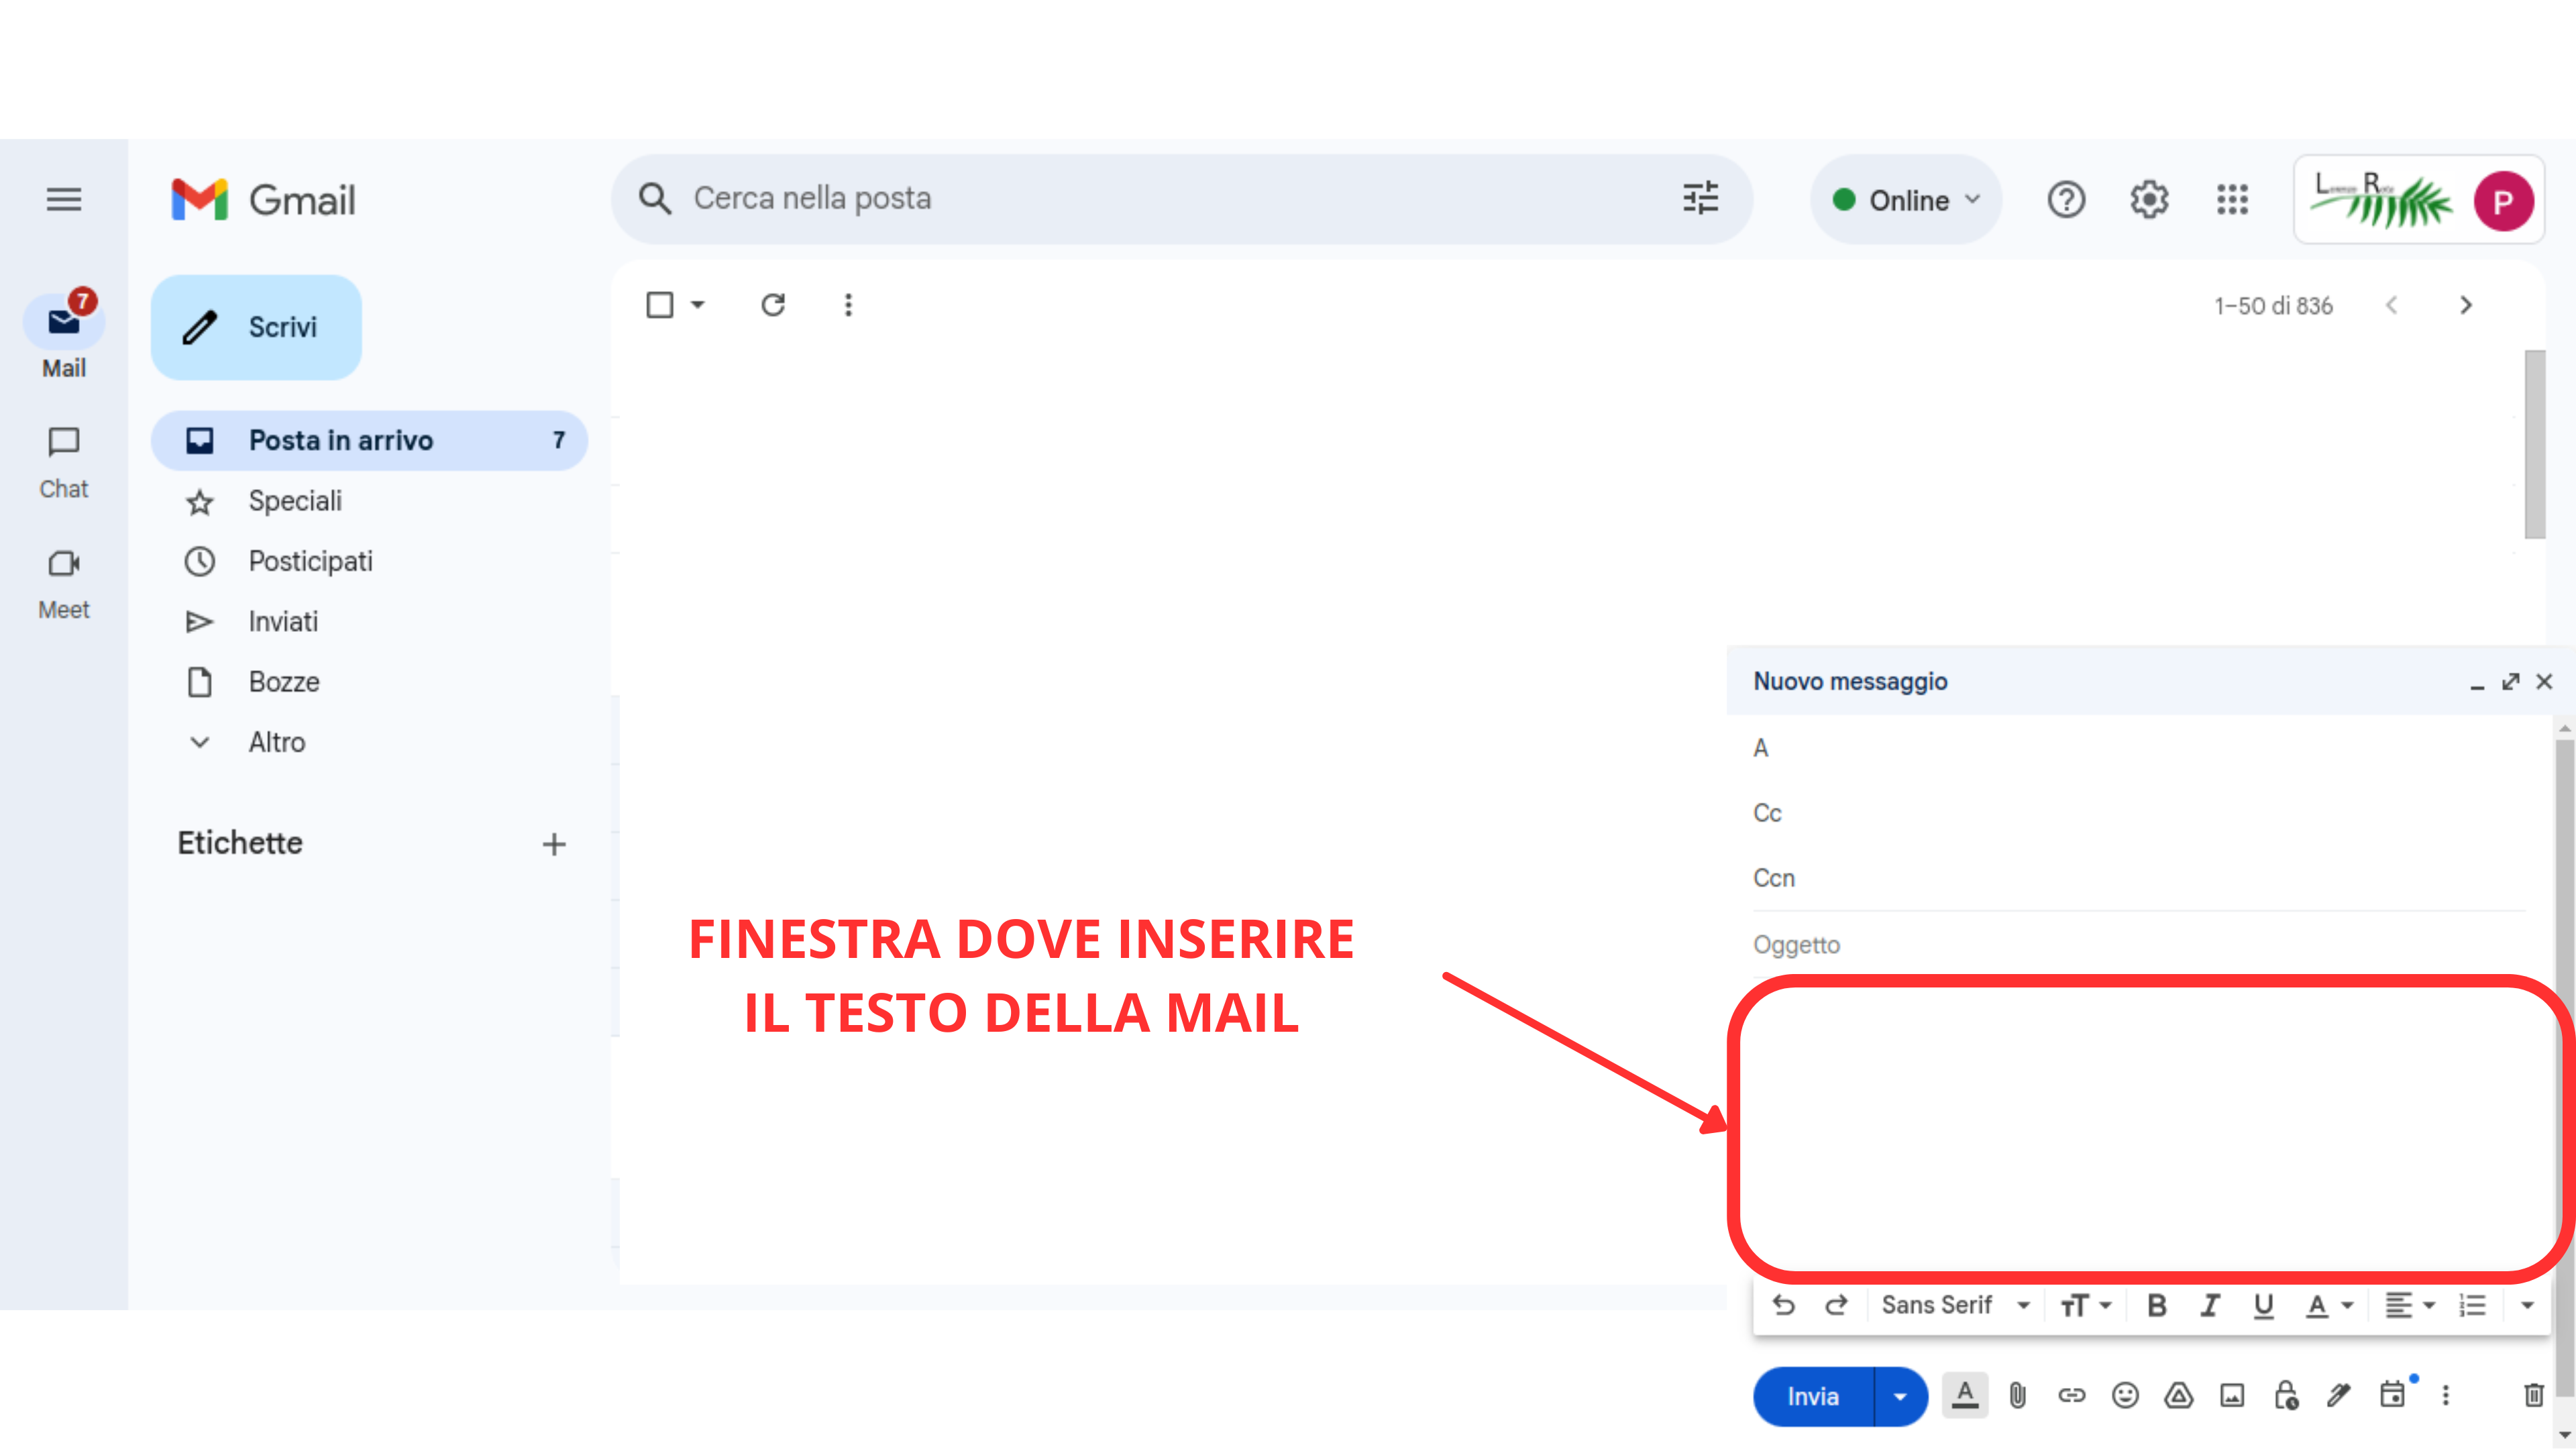
\includegraphics[width=\linewidth]{img/mail8.png}
        \caption{{screenshot della homepage di \href{https://mail.google.com/}{Google Mail}}, modificato con \href{https://www.canva.com}{Canva}}
    \end{figure}}
    \only<9>{\begin{figure}
        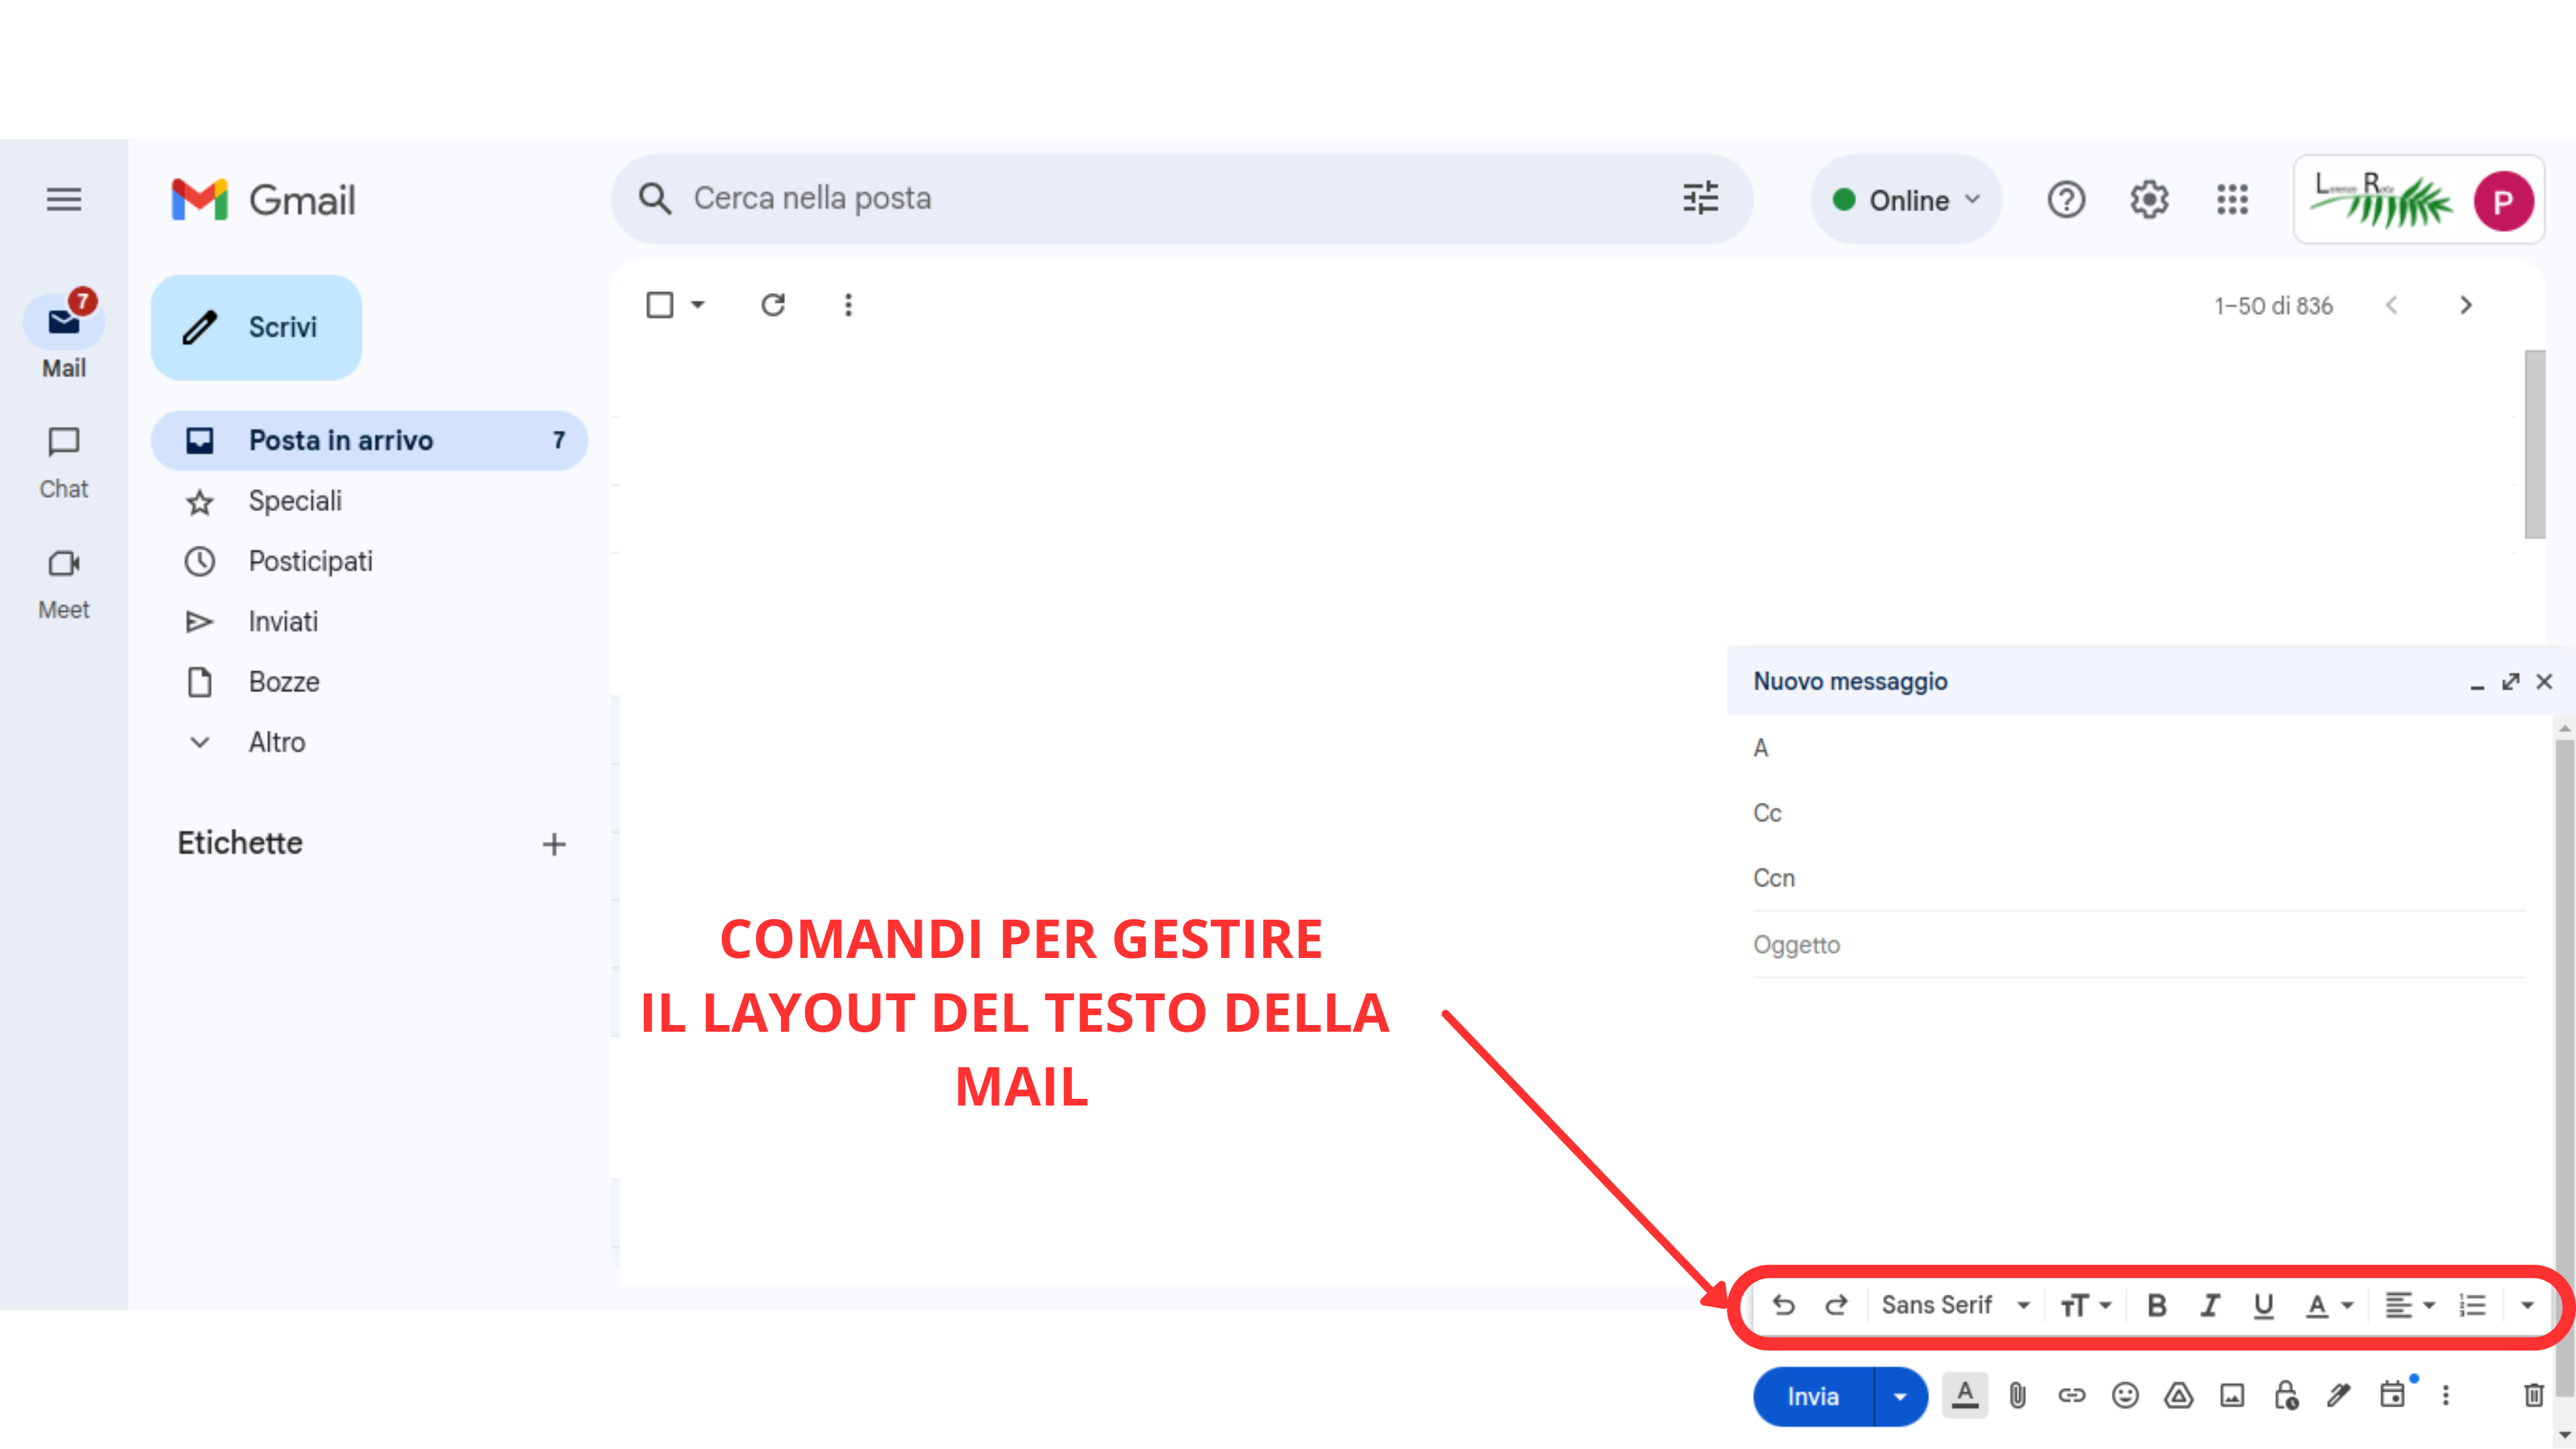
\includegraphics[width=\linewidth]{img/mail9.png}
        \caption{{screenshot della homepage di \href{https://mail.google.com/}{Google Mail}}, modificato con \href{https://www.canva.com}{Canva}}
    \end{figure}}
    \only<10>{\begin{figure}
        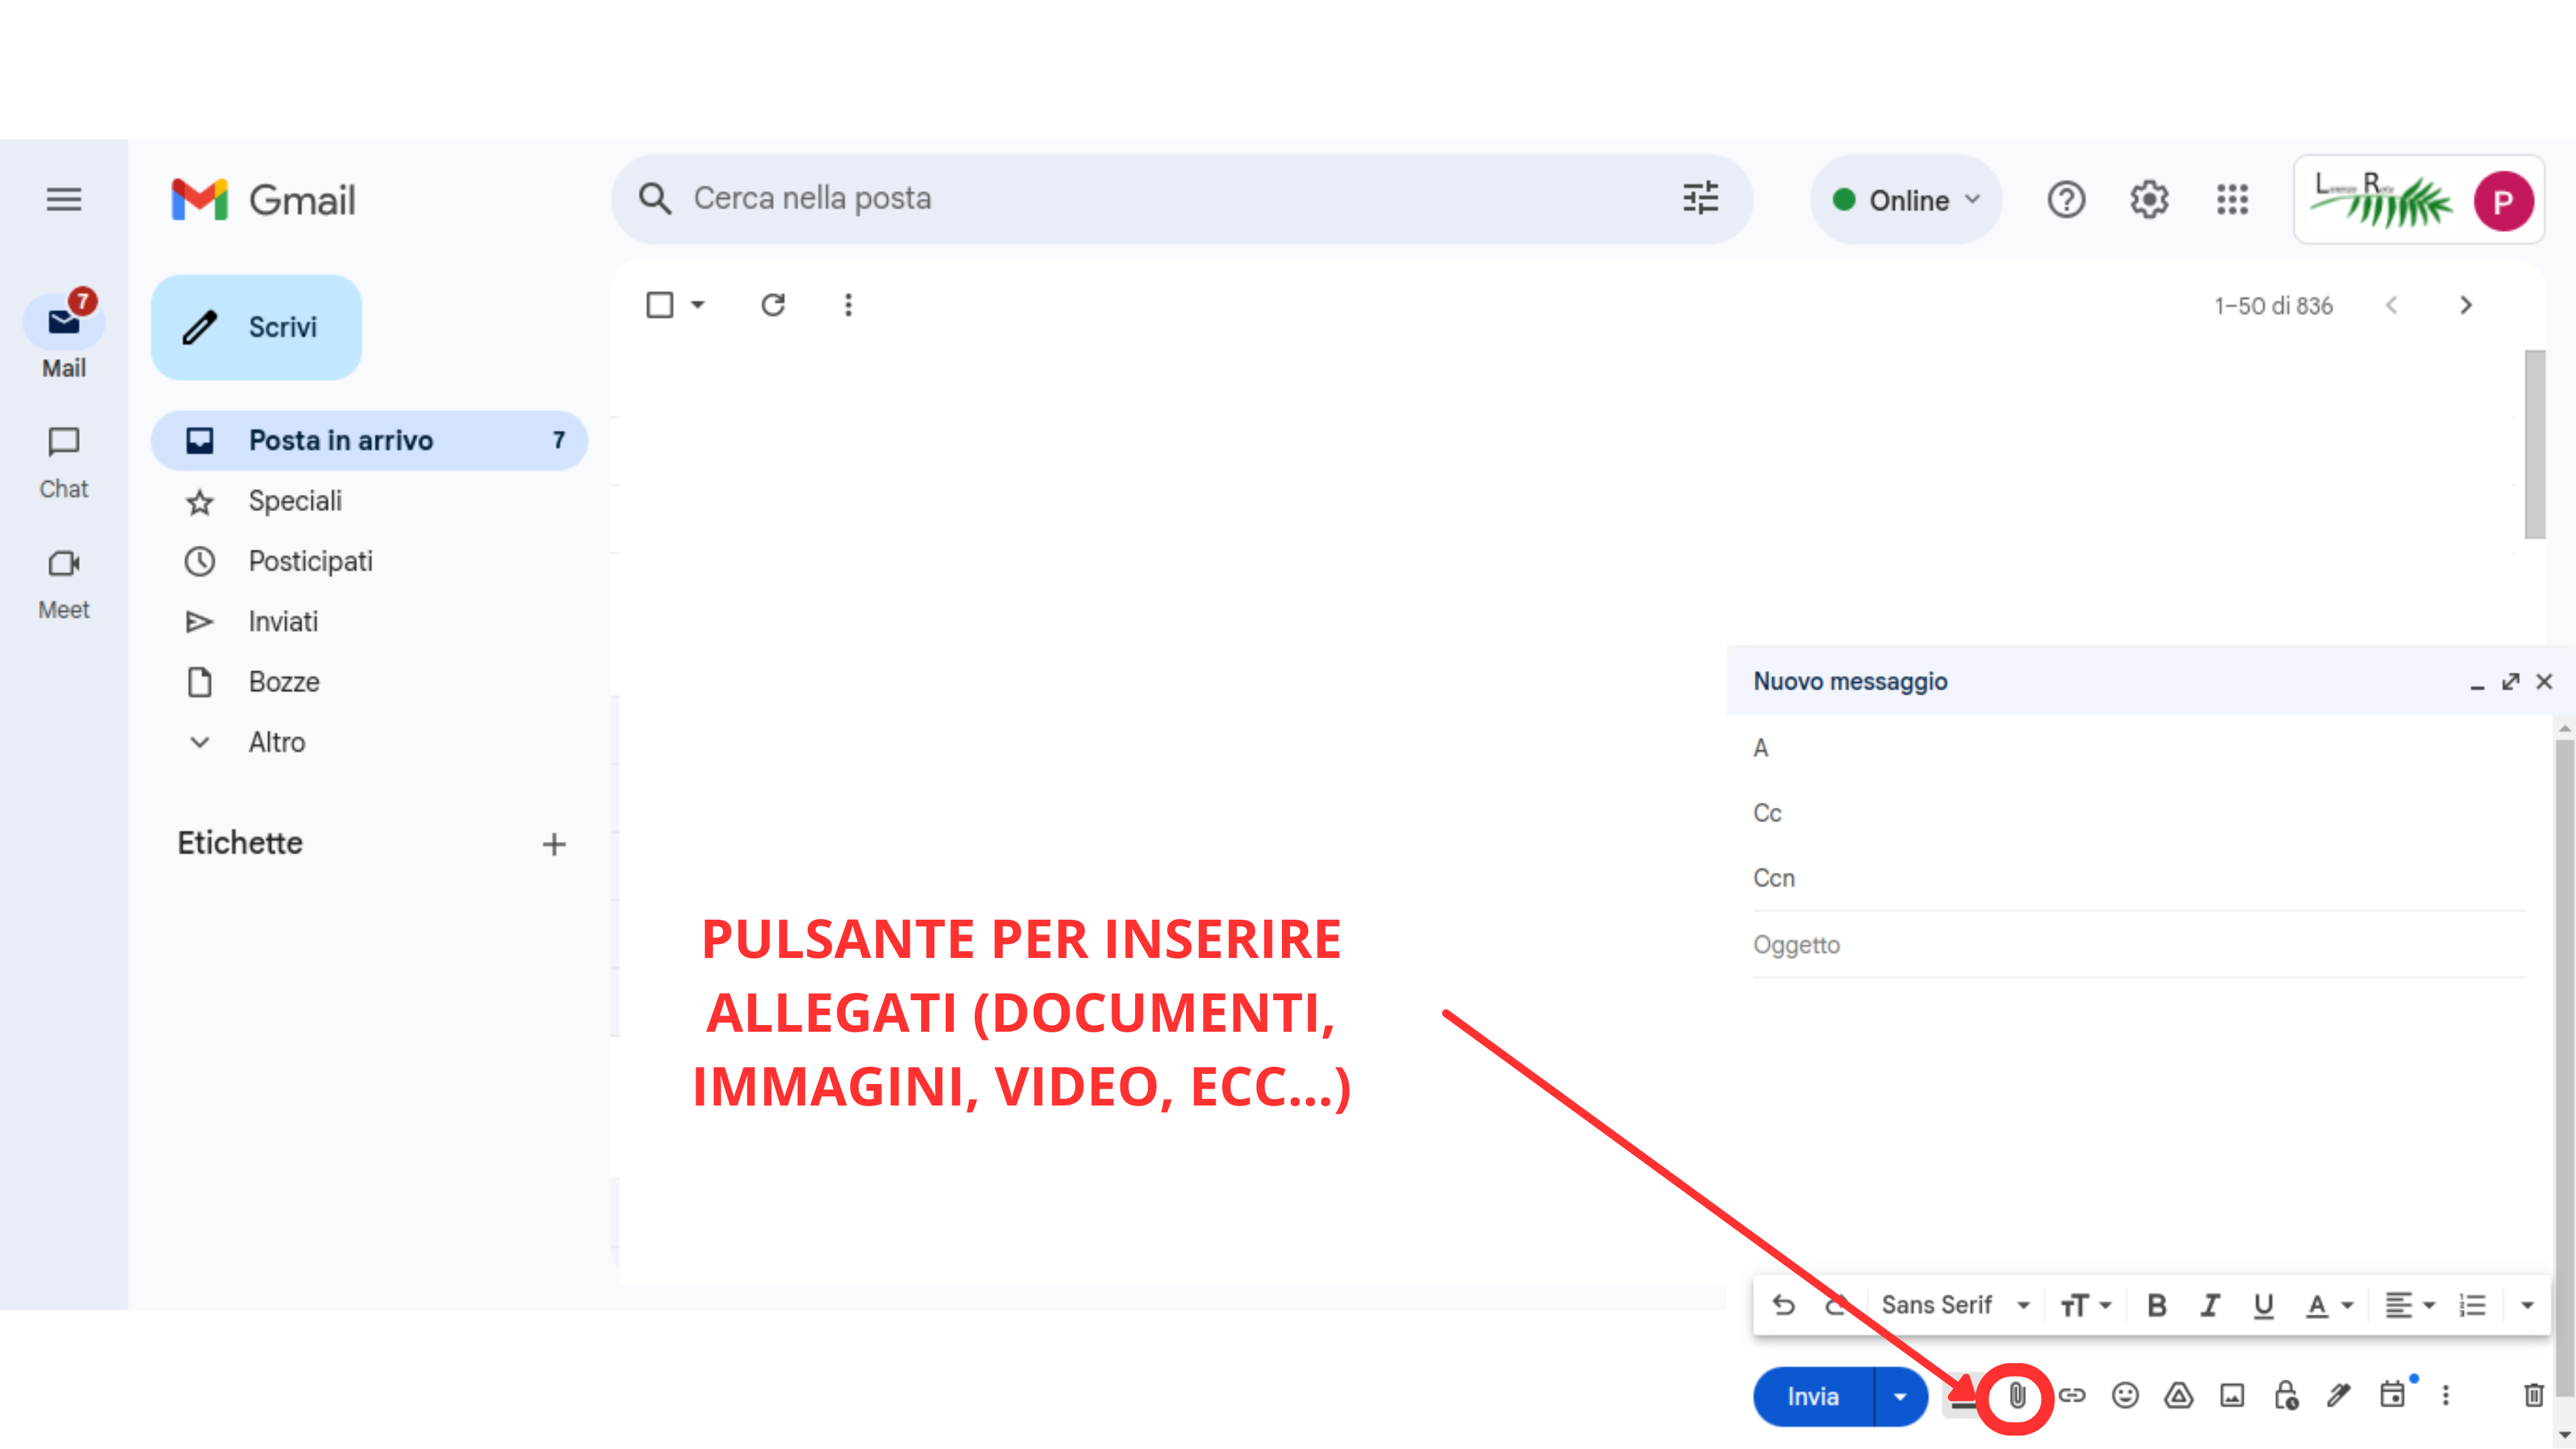
\includegraphics[width=\linewidth]{img/mail10.png}
        \caption{{screenshot della homepage di \href{https://mail.google.com/}{Google Mail}}, modificato con \href{https://www.canva.com}{Canva}}
    \end{figure}}
\end{frame}

\end{document}